\documentclass[12pt]{article}

% === [Packages] ===
\usepackage[utf8]{inputenc} % utf8 support
\usepackage[hmargin=1.25in,vmargin=1.25in]{geometry}
\usepackage{indentfirst}
\usepackage{lipsum}
\usepackage{url}
\usepackage[colorlinks,linkcolor=red!50!black,citecolor=blue!50!black,urlcolor=blue!50!black]{hyperref}
\usepackage{amsmath, amsfonts, amssymb}
\usepackage{pdfpages}
\usepackage{physics}
\usepackage{xcolor}
\usepackage{graphicx}
\usepackage{mathtools} % for the coloneq command
\usepackage{xparse}
\usepackage{ifthen} % For checking optional parameters
\usepackage{enumerate}
\usepackage{mathrsfs} % For \mathscr font
\usepackage{amsthm} % The AMS theorems package
\usepackage{tabularx}
\usepackage{authblk} % For affiliations

\usepackage{amsfonts}
\usepackage{indentfirst}
\usepackage{pgfplots}
\pgfplotsset{compat=1.16} % https://tex.stackexchange.com/questions/81899/what-does-running-in-backwards-compatibility-mode-mean-and-what-should-i-fix-t
\usepackage{tikz}

% === [amsthm declarations] ===
% http://www.math.ucsd.edu/~jeggers/latex/amsthdoc.pdf
%\swapnumbers
\newtheorem{thm}{Theorem}[section]
\newtheorem{prop}[thm]{Proposition}
\newtheorem{cor}{Corollary}[thm]
\newtheorem{lem}[thm]{Lemma}

\theoremstyle{definition}
\newtheorem{defn}{Definition}[section]
\theoremstyle{remark}
\newtheorem*{rem}{Remark}

\renewcommand{\qedsymbol}{$\blacksquare$}

% === [Misc] ===
% Multiple footnotes https://tex.stackexchange.com/questions/40072/incompatibility-between-footmisc-option-multiple-and-hyperref/62091#62091
\let\oldFootnote\footnote
\newcommand\nextToken\relax

\renewcommand\footnote[1]{%
    \oldFootnote{#1}\futurelet\nextToken\isFootnote}

\newcommand\isFootnote{%
    \ifx\footnote\nextToken\textsuperscript{,}\fi}

% === [global tikz configurations] ===
\usetikzlibrary{
    calc,
    arrows,
    shapes.geometric,
    intersections,
    pgfplots.fillbetween,
    decorations.pathreplacing,
    decorations.markings,
    patterns,
    cd % For commutative diagrams
}
\tikzcdset{% permits one to access the nodes in the tikzcd diagram by coordinate value, i.e. (m-1-2) or (m-4-3)
    every matrix/.append style={name=m},
}
\tikzset{% https://tex.stackexchange.com/questions/299149/adjunction-symbol-in-commutative-diagram
    symbol/.style={%
        draw=none,
        every to/.append style={%
            edge node={node [sloped, allow upside down, auto=false]{$#1$}}}
    }
}
\tikzset{every picture/.style={baseline={([yshift=-0.3em]current bounding box.center)}}}
\tikzset{
    % style to apply some styles to each segment of a path
    on each segment/.style={
        decorate,
        decoration={
            show path construction,
            moveto code={},
            lineto code={
                \path [#1]
                (\tikzinputsegmentfirst) -- (\tikzinputsegmentlast);
            },
            curveto code={
                \path [#1] (\tikzinputsegmentfirst)
                .. controls
                (\tikzinputsegmentsupporta) and (\tikzinputsegmentsupportb)
                ..
                (\tikzinputsegmentlast);
            },
            closepath code={
                \path [#1]
                (\tikzinputsegmentfirst) -- (\tikzinputsegmentlast);
            },
        },
    },
    % style to add short perpendicular bar midway along a path
    bar/.style={
        postaction={
            decorate,
            decoration={
                markings,
                mark=at position .5 with {\arrow{|}}
            }
        }
    },
    % style to add arrow half-way along an edge
    midarrow/.style={
        postaction={
            decorate,
            decoration={
                markings,
                mark=at position .5 with {\arrow{>}}
            }
        }
    }
}

% === [global notational macros] ===
\DeclareMathOperator{\id}{id}
\newcommand{\opcat}{\mathrm{op}}
\DeclareMathOperator{\Hom}{Hom}
\DeclareMathOperator{\cod}{cod}
\DeclareMathOperator{\dom}{dom}
\newcommand{\poly}{\mathsf{Poly}} % category of polyhedra and affine maps between them
\newcommand{\set}{\mathsf{Set}} % category of sets and functions between them
\newcommand{\cat}{\mathsf{Cat}} % 2-category of categories and functors between them and natural transformations between the functors
\newcommand{\sub}{\mathsf{Sub}} % the poset of subobjects and inclusions between them
\newcommand{\pow}{\mathsf{P}} % the powerset poset
\newcommand{\cone}{\mathsf{Cone}} % the powerset poset
\newcommand{\aff}{\mathsf{Aff}} % the category of affine spaces (?) and affine maps between them
\newcommand{\vect}{\mathsf{Vect}} % the category of vector spaces and linear maps between them
\newcommand{\mono}{\mathsf{Mono}} % the preorder of monomorphisms with shared codomain given by an argument
\newcommand{\arr}{\mathsf{Arr}} % the arrow category

\newcommand{\catA}{\mathcal{A}}
\newcommand{\catB}{\mathcal{B}}
\newcommand{\catC}{\mathcal{C}}
\newcommand{\catD}{\mathcal{D}}
\newcommand{\catE}{\mathcal{E}}

\newcommand{\Pf}{P}

% pullbacks are ubiquitous, here are macros for use inside a {tikzcd} environment
\newcommand{\drpb}[1]{\ar[dr, phantom, "\lrcorner", very near start, #1]}
\newcommand{\dlpb}[1]{\ar[dl, phantom, "\llcorner", very near start, #1]}
\newcommand{\urpb}[1]{\ar[ur, phantom, "\urcorner", very near start, #1]}
\newcommand{\ulpb}[1]{\ar[ul, phantom, "\ulcorner", very near start, #1]}

% given three coordinates, draw the pullback square between (#1) -- (#2) and (#1) -- (#3)
\newcommand{\pullback}[4][]{
    \coordinate (tmpbeg) at ($(#2)!1em!(#3)$);
    \coordinate (tmpend) at ($(#2)!1em!(#4)$);
    \coordinate (tmpmid) at ($(tmpbeg) + (tmpend) - (#2)$);
    \draw[#1] ($(tmpbeg)!0.3!(tmpmid)$) -- (tmpmid) -- ($(tmpend)!0.3!(tmpmid)$);
}

% The figure below demonstrates the usage of the pullback macros
% \begin{tikzcd}
%     ul & u & ur \\
%     l & a \ar[r] \ar[l] \ar[u] \ar[d] \drpb{} \drpb{shift={(+0.2,-0.2)}} \dlpb{red} \urpb{} \ulpb{} & r \\
%     dl & d & dr
% \end{tikzcd}

% === [Bibliography] ===
\usepackage[
    backend=biber,
    style=alphabetic,
]{biblatex}
\addbibresource{references.bib}

% === [Draft and writing tools] ===
\usepackage{showkeys}
\usepackage{todonotes}
\newcommand{\tob}[1]{\todo[color=blue!20,inline]{\textbf{Tobias:} #1}} % for comments by tobias
\newcommand{\tcf}[1]{\todo[color=green!20,inline]{\textbf{TC:} #1}} % for comments by tc
\newcommand{\ctodo}[1]{\todo[color=red!20,inline]{\textbf{TODO:} #1}} % generic todo

% === [Title page configuration] ===
\author[1,2]{Thomas C. Fraser}
\author[1]{Tobias Fritz}
\affil[1]{\textit{Perimeter Institute for Theoretical Physics, Waterloo, Ontario, Canada, N2L 2Y5}}
\affil[2]{\textit{Dept. of Physics and Astronomy, University of Waterloo, Waterloo, Ontario, Canada, N2L 3G1}}
\date{\today}
\title{On the Fibrations Underlying Optimization and Elimination}

% === [The document] ===
\begin{document}

\maketitle
\begin{abstract}
    \textit{As of July 25, 2019:} The theory of fibrations and fibered categories appears to be a natural place to discuss the theory of various optimization and elimination problems, including resolution in logic, linear and non-linear quantifier elimination, polytope projection, lattice optimization over various spaces, etc. These notes aim to investigate that claim and furthermore attempts to determine any and all structural similarities between the various cases.
\end{abstract}
\tableofcontents

\clearpage


\section*{Notation Proposals}
\begin{itemize}
    \item $\aff$ the category of affine spaces (?) and affine maps between them
    \item $\vect$ the category of vector spaces and the linear maps between them
    \item $\poly$ the category of polyhedra and the affine maps between them
    \item $\cone$ the category of cones and the linear maps between them
\end{itemize}

\section{Introduction}

Below is a provisional list of various notions of ``elimination'':

\begin{itemize} % indentation is messy here :(
    \item The \textbf{resolution rule} of propositional (and also first order) logics. Two clauses containing a complementary literals (e.g. variable $c$ in one and its negation $\neg c$ in the other) entails a clause with the complementary literals eliminated (see \textit{Ground resolvents and Ground resolution} in \cite{robinson1965machine}):\footnote{Reference \url{https://en.wikipedia.org/wiki/Resolution_(logic)}.}
        \[ \frac{a_1 \vee a_2 \vee \cdots \vee c, \quad b_1 \vee b_2 \vee \cdots \vee \neg c}{a_1 \vee a_2 \vee \cdots \vee b_1 \vee b_2 \vee \cdots} \]
    Equivalently,
        \[ \frac{(\neg a_1 \wedge \neg a_2 \wedge \cdots) \to c, \quad c \to (b_1 \vee b_2 \vee \cdots)}{(\neg a_1 \wedge \neg a_2 \wedge \cdots) \to (b_1 \vee b_2 \vee \cdots)} \]
    This generalizes to arbitrary conjunctions of literals which may or may not reference $c$ or $\neg c$.
    \item The incremental step of \textbf{Fourier-Motzkin elimination} \cite{ziegler2012lectures} for systems of linear inequalities. Given
        \[ a_0 + a_1 x_1 + a_2 x_2 + \cdots + a_n x_n \geq 0, \quad b_0 + b_1 x_1 + b_2 x_2 + \cdots + b_n x_n \geq 0 \]
    with $a_1 > 0$ and $b_1 < 0$, then
        \[ \left(\frac{a_0}{a_1} + \frac{a_2}{a_1} x_2 + \cdots + \frac{a_n}{a_1} x_n\right) - \left(\frac{b_0}{b_1} + \frac{b_2}{b_1} x_2 + \cdots + \frac{b_n}{b_1} x_n\right) \geq 0 \]
    This generalizes to arbitrary systems of linear inequalities over a set of variables containing $x_1$.
    \item The \textbf{elimination axiom of oriented matroids} \cite[circuit axiom (C3)]{bjorner1999oriented}. Given two citcuits $X_0 = (X_0^+, X_0^-), X_1 = (X_1^+, X_1^-)$ (with $X_0 \neq - X_1$), and an element $e \in X_0^+ \cap X_1^-$ which is positively oriented in one circuit and negatively oriented in the other, then the circuits can be ``glued'' along $e$ producing a new circuit $X = (X^+, X^-)$ satisfying  $X^+ \subseteq X_0^+ \cup X_1^+ \setminus \{e\}$ and $X^- \subseteq X_0^- \cup X_1^- \setminus \{e\}$ (i.e. it at least eliminates $e$). For example, the oriented matroid generated by the cycles of the following graph
    \begin{equation}
        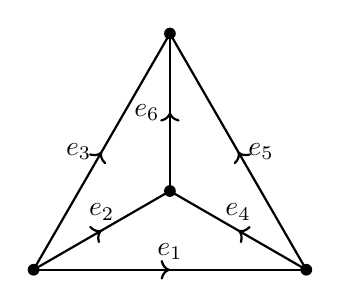
\begin{tikzpicture}
            \coordinate (v1) at (+210:2);
            \coordinate (v2) at (-30:2);
            \coordinate (v4) at (+90:2);
            \coordinate (v3) at (0,0);
            \foreach \v in {v1, v2, v3, v4} {
                \node at (\v)[circle, fill, inner sep=1.5pt]{};
            }
            \begin{scope}[thick]
                \draw[midarrow] (v1) -- node[left ]{$e_3$} (v4);
                \draw[midarrow] (v3) -- node[left ]{$e_6$} (v4);
                \draw[midarrow] (v1) -- node[above]{$e_2$} (v3);
                \draw[midarrow] (v1) -- node[above]{$e_1$} (v2);
                \draw[midarrow] (v2) -- node[right]{$e_5$} (v4);
                \draw[midarrow] (v2) -- node[above]{$e_4$} (v3);
            \end{scope}
        \end{tikzpicture}
    \end{equation}
    satisfies the elimination axiom. The following example eliminates $e_2$ (an indirectly eliminates $e_6$):
    \begin{equation}
        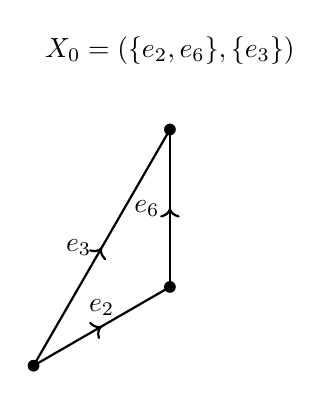
\begin{tikzpicture}
            \coordinate (v1) at (+210:2);
            \coordinate (v2) at (-30:2);
            \coordinate (v4) at (+90:2);
            \coordinate (v3) at (0,0);
            \foreach \v in {v1, v3, v4} {
                \node at (\v)[circle, fill, inner sep=1.5pt]{};
            }
            \begin{scope}[thick]
                \draw[midarrow] (v1) -- node[left ]{$e_3$} (v4);
                \draw[midarrow] (v3) -- node[left ]{$e_6$} (v4);
                \draw[midarrow] (v1) -- node[above]{$e_2$} (v3);
            \end{scope}
            \node at (0, 3)[]{$X_0 = (\{e_2, e_6\},\{e_3\})$};
        \end{tikzpicture}
        \qquad
        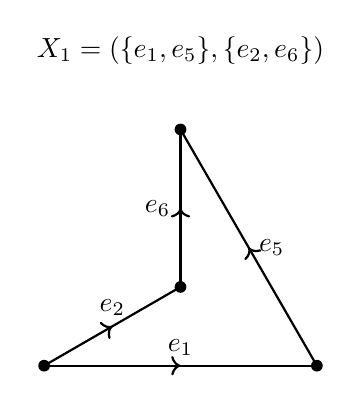
\begin{tikzpicture}
            \coordinate (v1) at (+210:2);
            \coordinate (v2) at (-30:2);
            \coordinate (v4) at (+90:2);
            \coordinate (v3) at (0,0);
            \foreach \v in {v1, v2, v3, v4} {
                \node at (\v)[circle, fill, inner sep=1.5pt]{};
            }
            \begin{scope}[thick]
                \draw[midarrow] (v3) -- node[left ]{$e_6$} (v4);
                \draw[midarrow] (v1) -- node[above]{$e_2$} (v3);
                \draw[midarrow] (v1) -- node[above]{$e_1$} (v2);
                \draw[midarrow] (v2) -- node[right]{$e_5$} (v4);
            \end{scope}
            \node at (0, 3)[]{$X_1 = (\{e_1, e_5\},\{e_2, e_6\})$};
        \end{tikzpicture}
        \qquad
        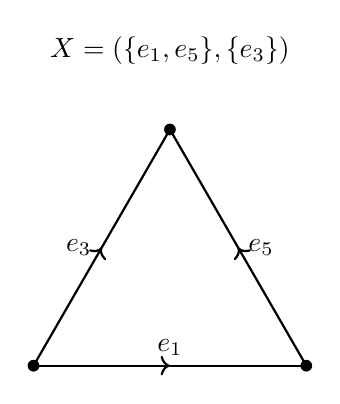
\begin{tikzpicture}
            \coordinate (v1) at (+210:2);
            \coordinate (v2) at (-30:2);
            \coordinate (v4) at (+90:2);
            \coordinate (v3) at (0,0);
            \foreach \v in {v1, v2, v4} {
                \node at (\v)[circle, fill, inner sep=1.5pt]{};
            }
            \begin{scope}[thick]
                \draw[midarrow] (v1) -- node[left ]{$e_3$} (v4);
                \draw[midarrow] (v1) -- node[above]{$e_1$} (v2);
                \draw[midarrow] (v2) -- node[right]{$e_5$} (v4);
            \end{scope}
            \node at (0, 3)[]{$X = (\{e_1, e_5\},\{e_3\})$};
        \end{tikzpicture}
    \end{equation}
    \tcf{Generally, this ``elimination'' of $n-1$ surfaces by gluing together $n$-dimensional surfaces reminds me of the analogous idea in the homology theory of polyhedra; assign to each $n$-dimensional face the sum of the $n-1$ faces \textit{incidence} to it (its boundary) as a formal sum in the free abelian group of all $n-1$ faces modulo $2$ (the modulo $2$ carries out the unoriented elimination). }
\end{itemize}

\section{Category Theory Terminology}

The following unordered list of categorical concepts are anticipated to be utilized:
\begin{itemize}
    \item adjunctions
    \item fibered categories
    \item cleavages
    \item pseudo functors (and if cleavages are splitting, functors)
    \item Beck-Chevalley condition
    \item Frobenius reciprocity (and functors of monoidal categories)
\end{itemize}

\tob{Cleavages are not really important because for any two different choices of cleavage, the resulting pullback functors are naturally isomorphic. So cleavages are just a technical tool relevant for proving the equivalence between fibred cats and pseudofunctors, but not relevant in practice}
\tcf{The above comment makes sense. Overall there are isomorphisms lurking behind every corner: first, there are natural isomorphisms present when considering the equivalence between pseudo-functors and "cleavaged" fibered categories, and second, whenever the cartesian arrows are indeed pullbacks, they are unique up to unique isomorphism and thus entire cleavages are unique up to unique isomorphisms. For a discussion see \cite{vistoli2004notes} at the end of Section 3.1.3. starting on page 50.}

\subsection{Cartesian Arrows}
\begin{defn}
    Let $P : \catE \to \catB$ be a functor between categories $\catE$ and $\catB$. An arrow $\phi : \alpha \to \beta$ of $\catE$ is \textit{cartesian} with respect to $P$ (sometimes \textit{$P$-cartesian}) if for every arrow $\psi : \gamma \to \beta$ sharing a codomain with $\phi$, and for every arrow $g : P(\gamma) \to P(\alpha)$ in $\catB$ satisfying $g \circ P(\phi) = P(\psi)$, there exists a unique arrow $\theta : \gamma \to \alpha$ in $\catE$ satisfying $\phi \circ \theta = \psi$ and $P(\theta) = g$.
    \begin{equation}
        \begin{tikzcd}[row sep=small]
            \gamma \arrow[rd, dashed, "\exists!\theta"'] \arrow[rrd, bend left, "\forall\psi"] \arrow[dd, mapsto] & & \\
            & \alpha \arrow[r, "\phi"'] & \beta \arrow[dd, mapsto] \\
            P(\gamma) \arrow[rd, "\forall g"'] \arrow[rrd, bend left, "P(\psi)"' near start] & & \\
            & P(\alpha) \arrow[r, "P(\phi)"'] \arrow[from=uu, mapsto, crossing over] & P(\beta)
        \end{tikzcd}
    \end{equation}
\end{defn}

\begin{cor}
    A cartesian morphism $\phi : \alpha \to \beta$ in $\catE$ with respect to a functor $P : \catE \to \catB$ establishes an isomorphism of categories \cite[Section~2.4.1]{lurie2009higher}\footnote{This formulation is also discussed here: \url{https://ncatlab.org/nlab/show/Cartesian+morphism\#CartInOrdCatReformulation}.}
    \begin{equation}
        \catE / \phi \cong \catE / \beta \times_{\catB / P(\beta)} \catB / P(\phi)
    \end{equation}
    where $\catE / \beta \times_{\catB / P(\beta)} \catB / P(\phi)$ is the pullback of functors.
    \begin{equation}
        \begin{tikzcd}
            \catE / \phi \ar[drr, bend left=20, "P/\phi"] \ar[ddr, bend right=40, "\mathrm{cod}"] \ar[dr, dashed, "\cong", leftrightarrow] & & \\
            & \catE / \beta \times_{\catB / P(\beta)} \catB / P(\phi) \ar[r] \ar[d] \drpb{xshift=-2em} & \catB / P(\phi) \ar[d, "\mathrm{cod}"] \\
            & \catE / \beta \ar[r, "P/\beta"] & \catB / P(\beta) \\
        \end{tikzcd}
    \end{equation}
\end{cor}

The pullback category $\catE / \beta \times_{\catB / P(\beta)} \catB / P(\phi)$ has morphisms associated with diagrams of $\catB$ with the following format:
\begin{equation}
    \begin{tikzcd}[row sep=large, column sep=small]
        & P(\gamma) \arrow[d, "P(\chi)"] \arrow[ddl, bend right, "f"'] \arrow[ddr, bend left, "P(\omega)"] & \\
        & P(\delta) \arrow[dl, "g"'] \arrow[dr, "P(\psi)"] & \\
        P(\alpha) \arrow[rr, "P(\phi)"] & & P(\beta)
    \end{tikzcd}
    \label{eq:pullback_category_cartesian}
\end{equation}
Evidently, if $\phi : \alpha \to \beta$ is cartesian, then there exists unique morphisms $\zeta : \gamma \to \alpha$ and $\eta : \delta \to \alpha$ such that $P(\zeta) = f$ and $P(\eta) = g$ and the following diagram of $\catE$ commutes:
\begin{equation}
    \begin{tikzcd}[row sep=large]
        & \gamma \arrow[d, "\chi"] \arrow[ddl, bend right, "\zeta"'] \arrow[ddr, bend left, "\omega"] & \\
        & \delta \arrow[dl, "\eta"'] \arrow[dr, "\psi"] & \\
        \alpha \arrow[rr, "\phi"] & & \beta
    \end{tikzcd}
    \label{eq:cartesian_over_category}
\end{equation}
Intuitively, if $\phi$ is cartesian, then in order to determine the category $\catE/\phi$ over $\phi$, it is sufficient to specify $\catE / \beta \times_{\catB / P(\beta)} \catB / P(\phi)$.

\subsection{Fibrations, Fibered Categories, and Cleavages}

\begin{defn}
    A \textit{fibered category over $\catB$} is a category $\catE$ associated to the domain of a functor, referred to as the \textit{fibration}, $P : \catE \to \catB$ with the property that for every morphism $f : a \to b$ of $\catB$ and object $\beta$ such that $P(\beta) = b$, there exists a cartesian arrow $\phi : \alpha \to \beta$ with $P(\phi) = f$.
\end{defn}

\begin{lem}
    A fibration $P : \catE \to \catB$ is a faithful functor if and only if its fibers are thin.
\end{lem}

\begin{proof}
    Recall that if $P : \catE \to \catB$ is a faithful functor, then by definition every pair of parallel arrows $\phi, \psi : \alpha \to \beta$ in $\catE$ satisfies
    \begin{equation}
        \label{eq:faithfulness}
        P(\phi) = P(\psi) : P(\alpha) \to P(\beta) \implies \phi = \psi.
    \end{equation}

    $\implies$ : Assuming $P : \catE \to \catB$ is faithful functor, consider an arbitrary pair of parallel arrows $\phi, \psi : \alpha \to \beta$ in an arbitrary fiber $\catE_{x}$ over $x$; i.e. $P(\phi) = P(\psi) = \id_{x}$. In such cases, faithfulness of $P$ (Eq.~\ref{eq:faithfulness}) guarantees that $\phi = \psi$ and thus $\catE_{x}$ is a thin category.

    $\impliedby$ : If the fiber $\catE_{x}$ for every object $x$ in $\catB$ is a thin category, then clearly $P : \catE \to \catB$ \textit{must} be faithful when restricted to an individual fiber. The non-trivial case is to consider an arbitrary pair of parallel morphisms $\phi, \psi : \alpha \to \beta$ not belonging to any fibers of $\catE$. Denote $a \coloneqq P(\alpha)$ and $b \coloneqq P(\beta)$ and suppose $f \coloneqq P(\phi) = P(\psi) : a \to b$. Then, because $\catE$ is a fibered category, there exists a cartesian arrow $\zeta : \gamma \to \beta$, such that $P(\zeta) = f$ (note that $a = P(\alpha) = P(\gamma)$ but $\gamma$ is not necessarily equal to $\alpha$). Since $\zeta$ is a cartesian arrow, there exists a unique arrows $\mu, \nu: \alpha \to \gamma$ completing the top edges of the following diagram:
    \begin{equation}
        \begin{tikzcd}
            \alpha \ar[dd, mapsto] \ar[rd, "\psi"', bend right] \ar[rr,dashed,"\mu"] & & \gamma \ar[dd, mapsto] \ar[ld, "\zeta"'] & \alpha \ar[dd, mapsto] \ar[lld, "\phi", bend left=20, crossing over, near start] \ar[l, dashed, "\nu"'] \\
            & \beta  & & \\
            a \ar[rr, equals] \ar[rd, "f"', bend right] & & a \ar[r, equals] \ar[ld, "f"] & a \ar[lld,"f", bend left=20] \\
            & b \ar[from=uu, mapsto, crossing over] & & \\
        \end{tikzcd}
        .
    \end{equation}
    However, $P(\nu) = \id_{a} = P(\mu)$ and therefore $\mu$ and $\nu$ are parallel arrows in the fiber $\catE_{a}$ and therefore $\mu = \nu$ because $\catE_{a}$ is assumed thin. Therefore, $\psi = \zeta \circ \mu = \zeta \circ \nu = \phi$ and thus $P$ is a faithful functor.
\end{proof}

\begin{defn}
    A \textit{cleavage} for a fibration $P : \catE \to \catB$ is an assignment to each morphism $f : a \to b$ of $\catB$ and object $\beta$ in $\catE_b$ (i.e. $P(\beta) = b$), a unique cartesian morphism $\kappa_{f}(B)$ of $\catE$ such that $P(\kappa_{f}(B)) = f$.
\end{defn}
Given a cleavage for a fibration, the cartesianness of morphisms within a cleavage permits one to establish functors between the fibers of the fibration. This concept is visualized in the following figure:

\begin{equation}
    \begin{tikzcd}[
            column sep=2em,
            execute at end picture={
                \fill[blue, opacity=0.1] (-7, -0.75) rectangle (+7, -1.5)
                    node[above left, blue!50!black, opacity=1]{$\catB$};
                \fill[red, opacity=0.1] (-7, +3.25) rectangle (+7, -0.25)
                    node[above left, red!50!black, opacity=1]{$\catE$};
                \fill[green, opacity=0.1] (-1.9, +2.25) rectangle (+1.9, +0.25)
                    node[above left, green!50!black, opacity=1]{$\catE_b$};
                \fill[green, opacity=0.1] (-6.9, +2.25) rectangle (-2.75, +0.25)
                    node[above left, green!50!black, opacity=1]{$\catE_a$};
                \fill[green, opacity=0.1] (+2.75, +2.25) rectangle (+6.9, +0.25)
                    node[above left, green!50!black, opacity=1]{$\catE_c$};
            }
        ]
        f^\ast\alpha
        \ar[rddd, mapsto, bend right]
        \ar[rr, "f^\ast(\phi\circ\psi)"', "(f^\ast\phi) \circ (f^\ast\psi)", dashed]
        \ar[rd, "f^\ast\psi"', dashed]
        & &
        f^\ast\beta
        \ar[lddd, mapsto, bend left]
        \ar[rrrr, "\kappa_f(\beta)", bend left]
        & &
        \alpha
        \ar[rddd, mapsto, bend right]
        \ar[rr, "\phi\circ \psi"]
        \ar[rd, "\psi"']
        \ar[from=llll, "\kappa_f(\alpha)", bend left, crossing over]
        \ar[from=rrrr, "\kappa_g(\alpha)"', bend right, crossing over]
        & &
        \beta
        \ar[lddd, mapsto, bend left]
        \ar[from=rrrr, "\kappa_g(\beta)"', bend right, crossing over]
        & &
        g^\ast\alpha
        \ar[rddd, mapsto, bend right]
        \ar[rr, "g^\ast(\phi\circ\psi)"', "(g^\ast\phi) \circ (g^\ast\psi)", dashed]
        \ar[rd, "g^\ast\psi"', dashed]
        & &
        g^\ast\beta
        \ar[lddd, mapsto, bend left]
        \\
        &
        f^\ast\gamma
        \ar[dd, mapsto]
        \ar[ru, "f^\ast\phi"', dashed]
        \ar[rrrr, "\kappa_f(\gamma)", bend right=10, crossing over]
        & & & &
        \gamma
        \ar[ru, "\phi"']
        \ar[dd, mapsto]
        & & & &
        g^\ast\gamma
        \ar[dd, mapsto]
        \ar[ru, "g^\ast\phi"', dashed]
        \ar[llll, "\kappa_g(\gamma)"', bend left=10, crossing over]
        &
        \\
        & & & & & & & & & &
        \\
        &
        a
        \ar[rrrr,"f"]
        & & & & b & & & &
        c
        \ar[llll, "g"']
        &
        \\
    \end{tikzcd}
\end{equation}

\subsection{Pseudo-Functors, Splitting Cleavages}

Pages 47-48 of \cite{vistoli2004notes} explicate the notions of pseudo-functors and their equivalence to fibrations with cleavages. Morover if the cleavage is splitting, the induced pseudo-functor is in fact a functor.

\subsection{Nearby Fibrations: Opfibrations and \texorpdfstring{$\ast$}{*}-fibrations}

Given a functor $P : \catE \to \catB$, it can be considered as a fibration in many different ways. For example, if $P^{\opcat} : \catE^{\opcat} \to \catB^{\opcat}$ is a fibration, then $P$ is said to be an \textit{opfibration}.

\subsection{Hom-Functors}
For a locally small category $\catC$, the hom-functor of $\catC$ is a functor $\Hom_{\catC} : \catC^{\opcat} \times \catC \to \set$ constructed in the following manner. Given objects $a,b,c,\ldots \in \catC_0$ of $\catC$, the hom-functor $\Hom_{\catC}$ maps a pair of objects $(a,b) \in (\catC^\opcat \times \catC)_0 = \catC_0 \times \catC_0 = \catC_0^2$ into the set\footnote{The collection of morphisms of type $a \to b$ forms a set because $\catC$ is locally small.} of morphisms $\catC_1$ of $\catC$ with source $a$ and target $b$. Therefore, $\Hom_{\catC}(a,b)$ is the set of morphisms in $\catC$ of type $a \to b$. Given morphisms $g^{\opcat} \in \Hom_{\catC^{\opcat}}(a,c)$ and $h \in \Hom_{\catC}(b,d)$, the hom-functor $\Hom_{\catC}$ constructs a function
\[ \Hom_{\catC}(g^{\opcat}, h) : \Hom_{\catC}(a,b) \to \Hom_{\catC}(c,d) \]
which takes a morphism $f : a \to b \in \Hom_{\catC}(a,b)$ and produces the morphism $h \circ f \circ g : c \to d \in \Hom_{\catC}(c,d)$. Graphically,
\[
    \Hom_{\catC}(g^{\opcat}, h)
    \left(
    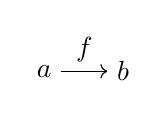
\begin{tikzpicture}
        \draw (0,0) node(a){$a$};
        \draw (1,0) node(b){$b$};
        \draw[->] (a) to node[above, midway]{$f$} (b);
    \end{tikzpicture}
    \right)
    =
    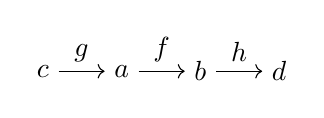
\begin{tikzpicture}
        \draw (0,0) node(c){$c$};
        \draw (1,0) node(a){$a$};
        \draw (2,0) node(b){$b$};
        \draw (3,0) node(d){$d$};
        \draw[->] (c) to node[above, midway]{$g$} (a);
        \draw[->] (a) to node[above, midway]{$f$} (b);
        \draw[->] (b) to node[above, midway]{$h$} (d);
    \end{tikzpicture}
\]

\subsection{Adjoint Functors}
Given two categories $\mathscr{C}$ and $\mathscr{D}$, a pair of functors $L : \mathscr C \to \mathscr D, R : \mathscr D \to \mathscr C$ are called an \textit{adjoint pair}, denoted $L \dashv R$ or
\[
    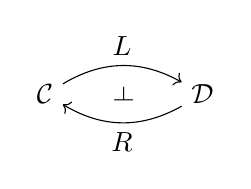
\begin{tikzpicture}
        \draw (0,0) node(c){$\catC$};
        \draw (2,0) node(d){$\catD$};
        \draw[->] (c) to[bend left] node[above, midway]{$L$} (d);
        \draw[->] (d) to[bend left] node[below, midway]{$R$} (c);
        \draw (1,0) node[rotate=-90]{$\dashv$};
    \end{tikzpicture}
\]
if there exists a natural isomorphism $\alpha$ between the following pair of hom-functors of type $\mathscr C^{\opcat} \times \mathscr D \to \set$:
\[ \Hom_{\mathscr D}(L^{\opcat}(-), -) \stackrel{\alpha}{\simeq} \Hom_{\mathscr C}(-, R(-)) \]
This relationship can be depicted graphically as $2$-cell (and its inverse) in $\cat$,
\[
    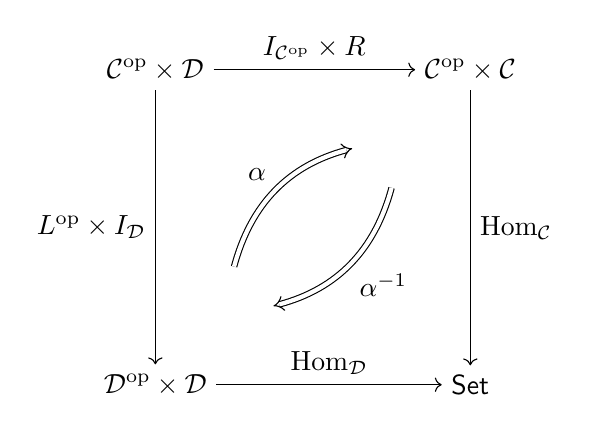
\begin{tikzpicture}
        \draw (0,4) node(tl){$\catC^\opcat \times \catD$};
        \draw (4,4) node(tr){$\catC^\opcat \times \catC$};

        \draw (0,0) node(bl){$\catD^{\opcat} \times \catD$};
        \draw (4,0) node(br){$\set$};
        \draw[->] (tl) to node[midway, above]{$I_{\catC^{\opcat}} \times R$} (tr);
        \draw[->] (bl) to node[midway, above]{$\Hom_{\catD}$} (br);
        \draw[->] (tl) to node[midway, left]{$L^{\opcat} \times I_{\catD}$} (bl);
        \draw[->] (tr) to node[midway, right]{$\Hom_{\catC}$} (br);

        \draw[double equal sign distance, -implies] (1,1.5) to[bend left] node[above left]{$\alpha$} (2.5,3);
        \draw[double equal sign distance, -implies] (3,2.5) to[bend left] node[below right]{$\alpha^{-1}$} (1.5,1);
    \end{tikzpicture}
\]
Concretely, the naturality of $\alpha$ means that for every morphism $(f^{\opcat} : b \to a, g : c \to d) \in (\catC^{\opcat} \times \catD)_1$ the components $\alpha_{(b,c)}$ and $\alpha_{(a,d)}$ of $\alpha$ make the following square commute:
\[
    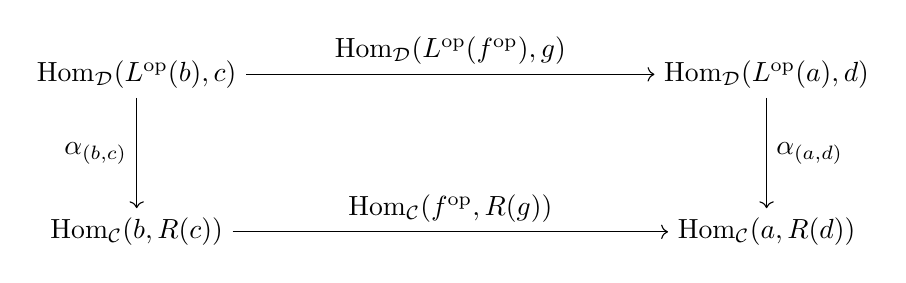
\begin{tikzpicture}
        \draw (0,2) node(tl){$\Hom_{\catD}(L^{\opcat}(b), c)$};
        \draw (8,2) node(tr){$\Hom_{\catD}(L^{\opcat}(a), d)$};
        \draw[->] (tl) to node[midway, above]{$\Hom_{\catD}(L^{\opcat}(f^{\opcat}), g)$} (tr);

        \draw (0,0) node(bl){$\Hom_{\catC}(b, R(c))$};
        \draw (8,0) node(br){$\Hom_{\catC}(a, R(d))$};
        \draw[->] (bl) to node[midway, above]{$\Hom_{\catC}(f^{\opcat}, R(g))$} (br);

        \draw[->] (tl) to node[midway, left]{$\alpha_{(b,c)}$} (bl);
        \draw[->] (tr) to node[midway, right]{$\alpha_{(a,d)}$} (br);
    \end{tikzpicture}
\]


\subsection{Beck-Chevalley Conditions}

The Beck-Chevalley Conditions are conditions that may or may not be satisfied by a quadruplet of functors $F,H,G,K$ which form a natural isomorphism $\alpha : K F \Rightarrow H G$ square:

\[
    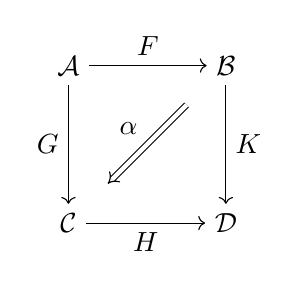
\begin{tikzpicture}
        \draw (-1,+1) node(tl){$\catA$};
        \draw (+1,+1) node(tr){$\catB$};
        \draw (-1,-1) node(bl){$\catC$};
        \draw (+1,-1) node(br){$\catD$};

        \draw[->] (tl) to node[above]{$F$} (tr);
        \draw[->] (tl) to node[left ]{$G$} (bl);
        \draw[->] (bl) to node[below]{$H$} (br);
        \draw[->] (tr) to node[right]{$K$} (br);

        \draw[double equal sign distance, -implies] (+0.5,+0.5) to node[above left]{$\alpha$} (-0.5,-0.5);
    \end{tikzpicture}
\]
To define the \textit{left} Beck-Chevalley condition, one needs functors $F_L : \catB \to \catA$ and $H_L : \catD \to \catA$ which are respectively left adjoint functors to $F$ and $H$,

\[
    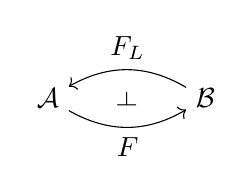
\begin{tikzpicture}
        \draw (-1,+1) node(tl){$\catA$};
        \draw (+1,+1) node(tr){$\catB$};

        \draw[->] (tl) to[bend right] node[below]{$F$} (tr);
        \draw[->] (tr) to[bend right] node[above]{$F_L$} (tl);
        \draw (0,+1) node[rotate=-90]{$\dashv$};
    \end{tikzpicture}
    ,
    \qquad
    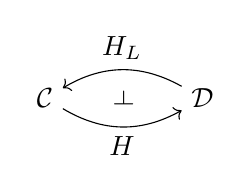
\begin{tikzpicture}
        \draw (-1,-1) node(bl){$\catC$};
        \draw (+1,-1) node(br){$\catD$};

        \draw[->] (bl) to[bend right] node[below]{$H$} (br);
        \draw[->] (br) to[bend right] node[above]{$H_L$} (bl);
        \draw (0,-1) node[rotate=-90]{$\dashv$};
    \end{tikzpicture}
    .
\]
Using these left adjoint functors, it becomes possible to construct a natural transformation $\beta : KH_L \Rightarrow GF_L$ from $\alpha$\footnote{The natural transformations $\alpha$ and $\beta$ are known as \textit{mates} or \textit{conjugates}.}. Graphically, $\beta$ can be identified as the outer cell of the following diagram:
\[
    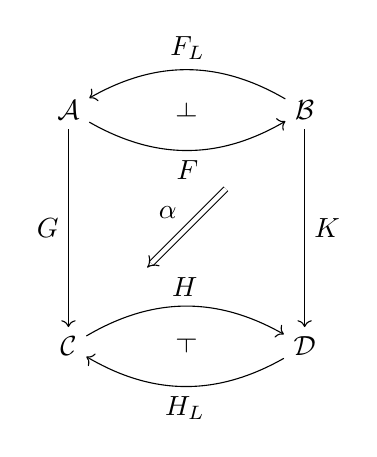
\begin{tikzpicture}
        \draw (-1.5,+1.5) node(tl){$\catA$};
        \draw (+1.5,+1.5) node(tr){$\catB$};
        \draw (-1.5,-1.5) node(bl){$\catC$};
        \draw (+1.5,-1.5) node(br){$\catD$};

        \draw[->] (tl) to[bend right] node[below]{$F$} (tr);
        \draw[->] (tr) to[bend right] node[above]{$F_L$} (tl);
        \draw (0,+1.5) node[rotate=-90]{$\dashv$};
        \draw[->] (tl) to node[left ]{$G$} (bl);
        \draw[->] (bl) to[bend left ] node[above]{$H$} (br);
        \draw[->] (br) to[bend left ] node[below]{$H_L$} (bl);
        \draw (0,-1.5) node[rotate=+90]{$\dashv$};
        \draw[->] (tr) to node[right]{$K$} (br);

        \draw[double equal sign distance, -implies] (+0.5,+0.5) to node[above left]{$\alpha$} (-0.5,-0.5);
    \end{tikzpicture},
    \qquad
    \text{i.e.}
    \qquad
    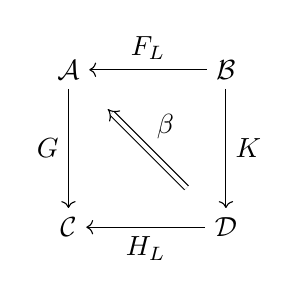
\begin{tikzpicture}
        \draw (-1,+1) node(tl){$\catA$};
        \draw (+1,+1) node(tr){$\catB$};
        \draw (-1,-1) node(bl){$\catC$};
        \draw (+1,-1) node(br){$\catD$};

        \draw[->] (tr) to node[above]{$F_L$} (tl);
        \draw[->] (tl) to node[left ]{$G$} (bl);
        \draw[->] (br) to node[below]{$H_L$} (bl);
        \draw[->] (tr) to node[right]{$K$} (br);

        \draw[double equal sign distance, -implies] (+0.5,-0.5) to node[above right]{$\beta$} (-0.5,+0.5);
    \end{tikzpicture}.
\]
Although the natural transformation $\alpha$ is assumed to be a natural isomorphism, the natural transformation $\beta$ need not be; if $\beta$ happens to be a natural isomorphism, then we say that the original square satisfies the \textit{left} Beck-Chevalley condition\footnote{Are the left adjoints $F_L, H_L$ unique? If not, it might be better to say the original square satifies the left Beck-Chevalley condition with respect to $F_L, H_L$.}. The \textit{right} Beck-Chevalley condition is defined analogously with functors $F_R, H_R$ which are respectively right adjoints $F \dashv F_R$ and $H \dashv H_R$.

\subsection{Slice and Coslice Categories}

Given a category $\catC$ and an object $c \in \catC_0$ of $\catC$, the \textit{slice category} (or \textit{over category}) $\catC/c$ is the ``stuff in $\catC$ that is on top of $c$''. Specifically, the objects of $\catC/c$ are all the morphisms $f \in \catC_1$ from $\catC$ whose codomain is $\cod(f) = c$ (alternatively you could write $(\catC/c)_0 = \Hom_{\catC}(-,c)$). A morphism of $\catC/c$ between objects $f : a \to c, g : b \to c \in (\catC/c)_0$ is a commuting triangle completed by a third morphism $h : a \to b \in \catC_1$:

\[
    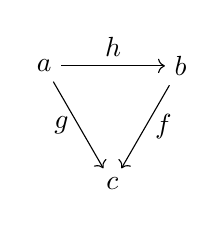
\begin{tikzpicture}
        \draw (150:1) node(tl){$a$};
        \draw ( 30:1) node(tr){$b$};
        \draw (270:1)node(bm){$c$};

        \draw[->] (tl) to node[below,left ]{$g$} (bm);
        \draw[->] (tr) to node[below,right]{$f$} (bm);

        \draw[->] (tl) to node[above]{$h$} (tr);
    \end{tikzpicture}
\]
Composition of morphisms in $\catC/c$ is induced by the composition of morphisms in $\catC$:
\[
    \left(
    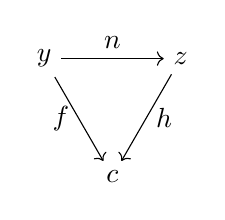
\begin{tikzpicture}
        \draw (150:1) node(tl){$y$};
        \draw ( 30:1) node(tr){$z$};
        \draw (270:1) node(bm){$c$};

        \draw[->] (tl) to node[below,left ]{$f$} (bm);
        \draw[->] (tr) to node[below,right]{$h$} (bm);

        \draw[->] (tl) to node[above]{$n$} (tr);
    \end{tikzpicture}
    \right)
    \circ_{\catC/c}
    \left(
    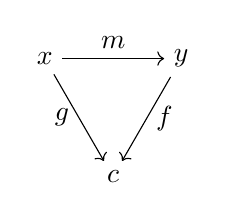
\begin{tikzpicture}
        \draw (150:1) node(tl){$x$};
        \draw ( 30:1) node(tr){$y$};
        \draw (270:1) node(bm){$c$};

        \draw[->] (tl) to node[below,left ]{$g$} (bm);
        \draw[->] (tr) to node[below,right]{$f$} (bm);

        \draw[->] (tl) to node[above]{$m$} (tr);
    \end{tikzpicture}
    \right)
    =
    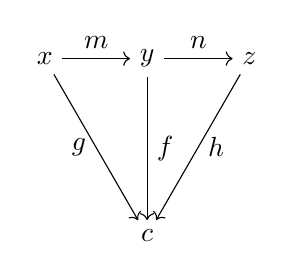
\begin{tikzpicture}
        \draw (150:1.5) node(tl){$x$};
        \draw ( 90:0.75) node(tm){$y$};
        \draw ( 30:1.5) node(tr){$z$};
        \draw (270:1.5) node(bm){$c$};

        \draw[->] (tl) to node[below,left ]{$g$} (bm);
        \draw[->] (tm) to node[right]{$f$} (bm);
        \draw[->] (tr) to node[below,right]{$h$} (bm);

        \draw[->] (tl) to node[above]{$m$} (tm);
        \draw[->] (tm) to node[above]{$n$} (tr);
    \end{tikzpicture}
\]

The assignment of an overcategory $\catC/c$ to each object $c$ can be extended to a \textit{slice functor} $\catC / (-) : \catC \to \mathbf{Cat}$ in the following sense. For objects $c \in \catC_0$, the slice functor takes $c$ to the slice category $\catC/c$; for morphisms $f : a \to b \in \catC_1$, the slice functor takes $f$ to the functor $\catC / f : \catC / a \to \catC / b$ defined graphically; for every morphism of $\catC / a$ (commuting triangle in $\catC$ over $a$), contruct the morphism of $\catC / b$ (commuting triangle in $\catC$ over $b$) as follows:
\[
    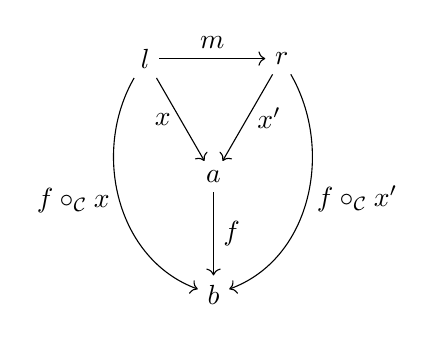
\begin{tikzpicture}
            \draw (150:1) node(tl){$l$};
            \draw ( 30:1) node(tr){$r$};
            \draw (270:1) node(bm){$a$};
            \draw (270:2.5) node(bb){$b$};

            \draw[->] (tl) to node[below,left ]{$x$}  (bm);
            \draw[->] (tr) to node[below,right]{$x'$} (bm);
            \draw[->] (tl) to[out=-120, in=+160] node[below,left ]{$f \circ_{\catC} x$}  (bb);
            \draw[->] (tr) to[out= -60, in= +20] node[below,right]{$f \circ_{\catC} x'$} (bb);
            \draw[->] (tl) to node[above]{$m$} (tr);
            \draw[->] (bm) to node[right]{$f$} (bb);
    \end{tikzpicture}
\]
where the inner triangle is a morphism of $\catC/a$ and the outer triangle is a morphism of $\catC/b$ given by the functor $\catC/f$.

Given a category $\catC$ and an object $c \in \catC_0$ of $\catC$ the \textit{coslice category} (or \textit{under category}) $c/\catC$ is the ``stuff in $\catC$ that is underneath $c$''. Specifically, the objects of $c/\catC$ are all the morphisms $f \in \catC_1$ from $\catC$ whose domain is $\dom(f) = c$ (alternatively you could write $(c/\catC)_0 = \Hom_{\catC}(c,-)$). A morphism of $c/\catC$ between objects $f : c \to a, g : c \to b \in (c/\catC)_0$ is a commuting triangle completed by a third morphism $h : a \to b \in \catC_1$:

\[
    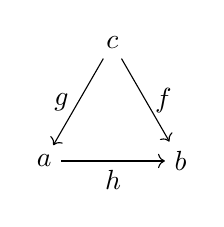
\begin{tikzpicture}
        \draw (210:1) node(tl){$a$};
        \draw (330:1) node(tr){$b$};
        \draw ( 90:1) node(bm){$c$};

        \draw[<-] (tl) to node[below,left ]{$g$} (bm);
        \draw[<-] (tr) to node[below,right]{$f$} (bm);
        \draw[->] (tl) to node[below]{$h$} (tr);
    \end{tikzpicture}
\]
Everything about coslice categories is defined as expected analogously to that of a slice categories.
\ctodo{determine how the details of the Grothendieck construction transform the slice (pseudo-)functor $\catC / (-) : \catC \to \mathbf{Cat}$ into the codomain fibration}
\subsection{Functors of Monoidal Categories}

\textcolor{red!50!black}{[TODO]}

\subsection{Frobenius Reciprocity}

\textcolor{red!50!black}{[TODO]}

\section{Case Studies of Interest}

\subsection{Polyhedra and Affine Maps}

One of the primary motiviating examples for this project is the theory of \textit{(finite) convex polyhedra} and the affine maps between them. Following \citeauthor{boyd2004convex}~\cite{boyd2004convex}, a \textit{polyhedron}\footnote{The term polytope will be reserved for the context of \textit{bounded polyhedron}. Note that the opposite convention is sometimes used by other authors as pointed out by \cite{boyd2004convex}.}\footnote{Alternative and sometimes inequivalent definitions for ``polyhedra'' do exist; oftentimes, these alternative definitions accomodate more general notions of polyhedra, such as non-convex polyhedra. Understanding the relationship between these various definitions, and the proposal of new ones, is a mathematical endeavour which dates back to antiquity and continues today  \cite{grunbaum2003your, lakatos2015proofs}.} $P$ is the intersection of a finite number of \textit{halfspaces} of some ambient vector space $V \cong \mathbb{R}^n$. A \textit{halfspace} $H \subseteq \mathbb{R}^n$ is a subset of a vector space (of dimension $n$) which is the solution set of a linear inequality constraint over canonical coordinates $x = (x_1, x_2, \ldots, x_n) \in \mathbb{R}^n$:
\begin{equation}
    H = \{ x \in V \mid a^\intercal x = \sum_{i=1}^{n} a_i x_i \geq b \}
\end{equation}

\begin{center}
    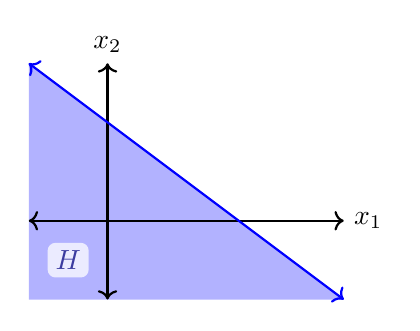
\begin{tikzpicture}[
            set label/.style={rounded corners=1mm, inner sep=1mm, fill=white, fill opacity=0.75}
        ]
        \coordinate (O) at (0,0);
        \coordinate (tl) at (-1,+2);
        \coordinate (br) at (+3,-1);
        \fill[blue, opacity=0.3] (tl) -- (br) -- (tl |- br) -- cycle;
        \draw[thick, <->] (O) ++(-1,0) -- ++(+4,0) node[right]{$x_1$};
        \draw[thick, <->] (O) ++(0,-1) -- ++(0,+3) node[above]{$x_2$};
        \draw[thick, blue, <->] (tl) -- (br);
        \node[blue!50!black, set label] at (-0.5, -0.5) {$H$};
        % \draw (+2.5, +0.5) node[]{$\mathbb{R}^2$};
    \end{tikzpicture}
\end{center}
As previously mentioned, a polyhedra is the intersection of finitely many halfspaces and therefore corresponds to
\begin{equation}
    P = \{ x \in V \mid \bigwedge_{j=1}^{k} (a_{j}^\intercal x \geq b_j) \}
\end{equation}

\begin{center}
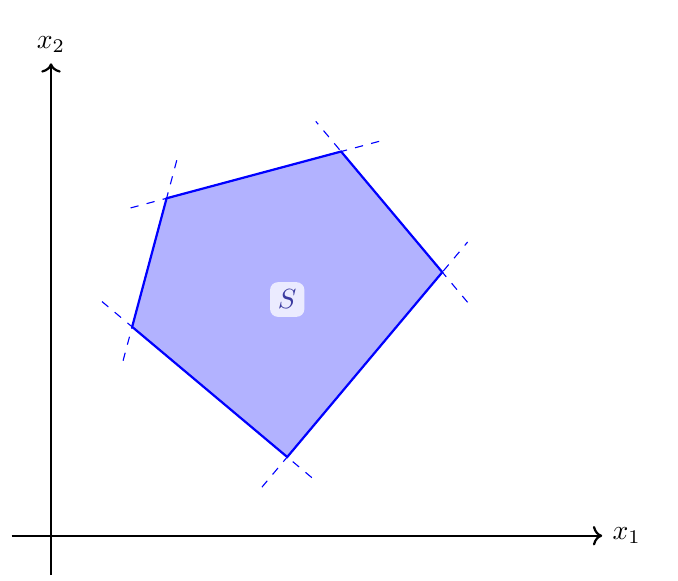
\begin{tikzpicture}[
        extend line/.style={dashed, shorten >= -0.5cm,shorten <= -0.5cm},
        set region/.style={fill=blue, fill opacity=0.3},
        set label/.style={rounded corners=1mm, inner sep=1mm, fill=white, fill opacity=0.75}
    ]
    \coordinate (ori) at (-3,-3);
    \coordinate (c1) at ($(ori)+(+7,0)$);
    \coordinate (c2) at ($(ori)+(0,+6)$);
    \draw[thick, ->, shorten <= -0.5cm] (ori) -- (c1) node[right]{$x_1$};
    \draw[thick, ->, shorten <= -0.5cm] (ori) -- (c2) node[above]{$x_2$};

    \coordinate (x1) at ( -90:2);
    \coordinate (x2) at ( +10:2);
    \coordinate (x3) at ( +70:2);
    \coordinate (x4) at (+140:2);
    \coordinate (x5) at (+190:2);
    % \foreach \p in {x1,x2,x3,x4,x5} {
    %     \node at (\p)[circle,fill,inner sep=1pt]{};
    % }
    \draw [blue, thick, set region] (x1) -- (x2) -- (x3) -- (x4) -- (x5) -- cycle;
    \foreach \p/\q in {x1/x2,x2/x3,x3/x4,x4/x5,x5/x1} {
        \draw [blue, extend line] (\p) -- (\q);
    }
    \node[blue!50!black, set label] at (0,0) {$S$};

\end{tikzpicture}
\end{center}

\begin{equation}
    \label{eq:pullback_of_positive_orthant}
    \begin{tikzcd}
        f^{\ast} ( \mathbb{R}^k_+ ) \ar[r, "f'"] \ar[d, hook, "j"] \drpb{xshift=-2mm} & \mathbb{R}^k_+ \ar[d, hook, "i"] \\
        \mathbb{R}^n \ar[r, "f"] & \mathbb{R}^k \\
    \end{tikzcd}
\end{equation}
In Equation~\ref{eq:pullback_of_positive_orthant}, the morphism $j$ is simply the inclusion of the polyhedra $f^\ast ( \mathbb{R}^k_+ )$ into its ambient vector space $\mathbb{R}^n$ and the morphism $f'$ is provided by the restriction of $f$ onto $f^\ast ( \mathbb{R}^k_+ )$.

\subsection{The Beck-Chevalley Condition for the Polyhedral Fibration}

Consider a commuting square of affine maps between vector spaces in the base category of affine maps

\begin{defn}
    The category $\poly$ consists of polyhedra as objects and affine maps between them.
\end{defn}
\begin{center}
    \newcommand{\importpolyproj}[1]{
    \begin{tikzpicture}[
            scale=0.6,
            line join=round,
            poly_vertex/.style = {circle,fill,blue,inner sep=0.75pt},
            poly_edge/.style = {thick, blue},
            poly_face/.style = {blue, opacity=0.15}
        ]
        \coordinate (O) at (0,0,0);
        \coordinate (x1) at (5,0,0);
        \coordinate (x2) at (0,5,0);
        \coordinate (x3) at (0,0,5);
        \draw[thick, ->] (O) -- (x1) node[right]{$x$};
        \draw[thick, ->] (O) -- (x2) node[above]{$y$};
        \draw[thick, ->] (O) -- (x3) node[left]{$z$};
        #1
    \end{tikzpicture}
    }
    \importpolyproj{\coordinate (v1) at (1.62362,3.,3.26287);
\node at (v1) [poly_vertex]{};
\coordinate (v2) at (4.37638,3.,2.73713);
\node at (v2) [poly_vertex]{};
\coordinate (v3) at (2.57467,1.69098,3.26287);
\node at (v3) [poly_vertex]{};
\coordinate (v4) at (2.57467,4.30902,3.26287);
\node at (v4) [poly_vertex]{};
\coordinate (v5) at (4.11352,2.19098,3.26287);
\node at (v5) [poly_vertex]{};
\coordinate (v6) at (4.11352,3.80902,3.26287);
\node at (v6) [poly_vertex]{};
\coordinate (v7) at (2.73713,2.19098,4.11352);
\node at (v7) [poly_vertex]{};
\coordinate (v8) at (2.73713,3.80902,4.11352);
\node at (v8) [poly_vertex]{};
\coordinate (v9) at (2.31181,2.5,1.88648);
\node at (v9) [poly_vertex]{};
\coordinate (v10) at (2.31181,3.5,1.88648);
\node at (v10) [poly_vertex]{};
\coordinate (v11) at (3.68819,2.5,4.11352);
\node at (v11) [poly_vertex]{};
\coordinate (v12) at (3.68819,3.5,4.11352);
\node at (v12) [poly_vertex]{};
\coordinate (v13) at (3.85065,3.,1.88648);
\node at (v13) [poly_vertex]{};
\coordinate (v14) at (1.88648,2.19098,2.73713);
\node at (v14) [poly_vertex]{};
\coordinate (v15) at (1.88648,3.80902,2.73713);
\node at (v15) [poly_vertex]{};
\coordinate (v16) at (2.14935,3.,4.11352);
\node at (v16) [poly_vertex]{};
\coordinate (v17) at (3.26287,2.19098,1.88648);
\node at (v17) [poly_vertex]{};
\coordinate (v18) at (3.26287,3.80902,1.88648);
\node at (v18) [poly_vertex]{};
\coordinate (v19) at (3.42533,1.69098,2.73713);
\node at (v19) [poly_vertex]{};
\coordinate (v20) at (3.42533,4.30902,2.73713);
\node at (v20) [poly_vertex]{};
\draw[poly_edge] (v1) -- (v14);
\draw[poly_edge] (v1) -- (v15);
\draw[poly_edge] (v1) -- (v16);
\draw[poly_edge] (v2) -- (v5);
\draw[poly_edge] (v2) -- (v6);
\draw[poly_edge] (v2) -- (v13);
\draw[poly_edge] (v3) -- (v7);
\draw[poly_edge] (v3) -- (v14);
\draw[poly_edge] (v3) -- (v19);
\draw[poly_edge] (v4) -- (v8);
\draw[poly_edge] (v4) -- (v15);
\draw[poly_edge] (v4) -- (v20);
\draw[poly_edge] (v5) -- (v11);
\draw[poly_edge] (v5) -- (v19);
\draw[poly_edge] (v6) -- (v12);
\draw[poly_edge] (v6) -- (v20);
\draw[poly_edge] (v7) -- (v11);
\draw[poly_edge] (v7) -- (v16);
\draw[poly_edge] (v8) -- (v12);
\draw[poly_edge] (v8) -- (v16);
\draw[poly_edge] (v9) -- (v10);
\draw[poly_edge] (v9) -- (v14);
\draw[poly_edge] (v9) -- (v17);
\draw[poly_edge] (v10) -- (v15);
\draw[poly_edge] (v10) -- (v18);
\draw[poly_edge] (v11) -- (v12);
\draw[poly_edge] (v13) -- (v17);
\draw[poly_edge] (v13) -- (v18);
\draw[poly_edge] (v17) -- (v19);
\draw[poly_edge] (v18) -- (v20);
\fill[poly_face] (v15) -- (v10) -- (v9) -- (v14) -- (v1) -- cycle;
\fill[poly_face] (v2) -- (v6) -- (v12) -- (v11) -- (v5) -- cycle;
\fill[poly_face] (v5) -- (v11) -- (v7) -- (v3) -- (v19) -- cycle;
\fill[poly_face] (v11) -- (v12) -- (v8) -- (v16) -- (v7) -- cycle;
\fill[poly_face] (v12) -- (v6) -- (v20) -- (v4) -- (v8) -- cycle;
\fill[poly_face] (v6) -- (v2) -- (v13) -- (v18) -- (v20) -- cycle;
\fill[poly_face] (v2) -- (v5) -- (v19) -- (v17) -- (v13) -- cycle;
\fill[poly_face] (v4) -- (v20) -- (v18) -- (v10) -- (v15) -- cycle;
\fill[poly_face] (v18) -- (v13) -- (v17) -- (v9) -- (v10) -- cycle;
\fill[poly_face] (v17) -- (v19) -- (v3) -- (v14) -- (v9) -- cycle;
\fill[poly_face] (v3) -- (v7) -- (v16) -- (v1) -- (v14) -- cycle;
\fill[poly_face] (v16) -- (v8) -- (v4) -- (v15) -- (v1) -- cycle;
\coordinate (p121) at (1.62362,3.,0.);
\node at (p121) [poly_vertex]{};
\coordinate (p122) at (4.37638,3.,0.);
\node at (p122) [poly_vertex]{};
\coordinate (p123) at (2.57467,1.69098,0.);
\node at (p123) [poly_vertex]{};
\coordinate (p124) at (2.57467,4.30902,0.);
\node at (p124) [poly_vertex]{};
\coordinate (p125) at (4.11352,2.19098,0.);
\node at (p125) [poly_vertex]{};
\coordinate (p126) at (4.11352,3.80902,0.);
\node at (p126) [poly_vertex]{};
\coordinate (p127) at (1.88648,2.19098,0.);
\node at (p127) [poly_vertex]{};
\coordinate (p128) at (1.88648,3.80902,0.);
\node at (p128) [poly_vertex]{};
\coordinate (p129) at (3.42533,1.69098,0.);
\node at (p129) [poly_vertex]{};
\coordinate (p1210) at (3.42533,4.30902,0.);
\node at (p1210) [poly_vertex]{};
\draw[poly_edge] (p121) -- (p127);
\draw[poly_edge] (p127) -- (p123);
\draw[poly_edge] (p123) -- (p129);
\draw[poly_edge] (p129) -- (p125);
\draw[poly_edge] (p125) -- (p122);
\draw[poly_edge] (p122) -- (p126);
\draw[poly_edge] (p126) -- (p1210);
\draw[poly_edge] (p1210) -- (p124);
\draw[poly_edge] (p124) -- (p128);
\draw[poly_edge] (p128) -- (p121);
\fill[poly_face] (p121) -- (p127) -- (p123) -- (p129) -- (p125) -- (p122) -- (p126) -- (p1210) -- (p124) -- (p128) -- cycle;
\coordinate (p231) at (0.,1.69098,3.26287);
\node at (p231) [poly_vertex]{};
\coordinate (p232) at (0.,4.30902,3.26287);
\node at (p232) [poly_vertex]{};
\coordinate (p233) at (0.,2.19098,4.11352);
\node at (p233) [poly_vertex]{};
\coordinate (p234) at (0.,3.80902,4.11352);
\node at (p234) [poly_vertex]{};
\coordinate (p235) at (0.,2.5,1.88648);
\node at (p235) [poly_vertex]{};
\coordinate (p236) at (0.,3.5,1.88648);
\node at (p236) [poly_vertex]{};
\coordinate (p237) at (0.,2.5,4.11352);
\node at (p237) [poly_vertex]{};
\coordinate (p238) at (0.,3.5,4.11352);
\node at (p238) [poly_vertex]{};
\coordinate (p239) at (0.,3.,1.88648);
\node at (p239) [poly_vertex]{};
\coordinate (p2310) at (0.,3.,4.11352);
\node at (p2310) [poly_vertex]{};
\coordinate (p2311) at (0.,2.19098,1.88648);
\node at (p2311) [poly_vertex]{};
\coordinate (p2312) at (0.,3.80902,1.88648);
\node at (p2312) [poly_vertex]{};
\coordinate (p2313) at (0.,1.69098,2.73713);
\node at (p2313) [poly_vertex]{};
\coordinate (p2314) at (0.,4.30902,2.73713);
\node at (p2314) [poly_vertex]{};
\draw[poly_edge] (p231) -- (p2313);
\draw[poly_edge] (p2313) -- (p2311);
\draw[poly_edge] (p2311) -- (p235);
\draw[poly_edge] (p235) -- (p239);
\draw[poly_edge] (p239) -- (p236);
\draw[poly_edge] (p236) -- (p2312);
\draw[poly_edge] (p2312) -- (p2314);
\draw[poly_edge] (p2314) -- (p232);
\draw[poly_edge] (p232) -- (p234);
\draw[poly_edge] (p234) -- (p238);
\draw[poly_edge] (p238) -- (p2310);
\draw[poly_edge] (p2310) -- (p237);
\draw[poly_edge] (p237) -- (p233);
\draw[poly_edge] (p233) -- (p231);
\fill[poly_face] (p231) -- (p2313) -- (p2311) -- (p235) -- (p239) -- (p236) -- (p2312) -- (p2314) -- (p232) -- (p234) -- (p238) -- (p2310) -- (p237) -- (p233) -- cycle;
\coordinate (p131) at (1.62362,0.,3.26287);
\node at (p131) [poly_vertex]{};
\coordinate (p132) at (4.37638,0.,2.73713);
\node at (p132) [poly_vertex]{};
\coordinate (p133) at (4.11352,0.,3.26287);
\node at (p133) [poly_vertex]{};
\coordinate (p134) at (2.73713,0.,4.11352);
\node at (p134) [poly_vertex]{};
\coordinate (p135) at (2.31181,0.,1.88648);
\node at (p135) [poly_vertex]{};
\coordinate (p136) at (3.68819,0.,4.11352);
\node at (p136) [poly_vertex]{};
\coordinate (p137) at (3.85065,0.,1.88648);
\node at (p137) [poly_vertex]{};
\coordinate (p138) at (1.88648,0.,2.73713);
\node at (p138) [poly_vertex]{};
\coordinate (p139) at (2.14935,0.,4.11352);
\node at (p139) [poly_vertex]{};
\coordinate (p1310) at (3.26287,0.,1.88648);
\node at (p1310) [poly_vertex]{};
\draw[poly_edge] (p131) -- (p138);
\draw[poly_edge] (p138) -- (p135);
\draw[poly_edge] (p135) -- (p1310);
\draw[poly_edge] (p1310) -- (p137);
\draw[poly_edge] (p137) -- (p132);
\draw[poly_edge] (p132) -- (p133);
\draw[poly_edge] (p133) -- (p136);
\draw[poly_edge] (p136) -- (p134);
\draw[poly_edge] (p134) -- (p139);
\draw[poly_edge] (p139) -- (p131);
\fill[poly_face] (p131) -- (p138) -- (p135) -- (p1310) -- (p137) -- (p132) -- (p133) -- (p136) -- (p134) -- (p139) -- cycle;
\coordinate (p11) at (1.62362,0.,0.);
\node at (p11) [poly_vertex]{};
\coordinate (p12) at (4.37638,0.,0.);
\node at (p12) [poly_vertex]{};
\draw[poly_edge] (p11) -- (p12);

\coordinate (p21) at (0.,1.69098,0.);
\node at (p21) [poly_vertex]{};
\coordinate (p22) at (0.,4.30902,0.);
\node at (p22) [poly_vertex]{};
\draw[poly_edge] (p21) -- (p22);

\coordinate (p31) at (0.,0.,1.88648);
\node at (p31) [poly_vertex]{};
\coordinate (p32) at (0.,0.,4.11352);
\node at (p32) [poly_vertex]{};
\draw[poly_edge] (p31) -- (p32);
}
    \importpolyproj{\coordinate (v1) at (1.61791,2.77261,3.19526);
\node at (v1) [poly_vertex]{};
\coordinate (v2) at (2.80474,4.38209,3.22739);
\node at (v2) [poly_vertex]{};
\coordinate (v3) at (2.77261,3.19526,1.61791);
\node at (v3) [poly_vertex]{};
\coordinate (v4) at (3.22739,2.80474,4.38209);
\node at (v4) [poly_vertex]{};
\coordinate (v5) at (3.19526,1.61791,2.77261);
\node at (v5) [poly_vertex]{};
\coordinate (v6) at (4.38209,3.22739,2.80474);
\node at (v6) [poly_vertex]{};
\draw[poly_edge] (v1) -- (v2);
\draw[poly_edge] (v1) -- (v3);
\draw[poly_edge] (v1) -- (v4);
\draw[poly_edge] (v1) -- (v5);
\draw[poly_edge] (v2) -- (v3);
\draw[poly_edge] (v2) -- (v4);
\draw[poly_edge] (v2) -- (v6);
\draw[poly_edge] (v3) -- (v5);
\draw[poly_edge] (v3) -- (v6);
\draw[poly_edge] (v4) -- (v5);
\draw[poly_edge] (v4) -- (v6);
\draw[poly_edge] (v5) -- (v6);
\fill[poly_face] (v4) -- (v5) -- (v6) -- cycle;
\fill[poly_face] (v4) -- (v6) -- (v2) -- cycle;
\fill[poly_face] (v4) -- (v2) -- (v1) -- cycle;
\fill[poly_face] (v4) -- (v1) -- (v5) -- cycle;
\fill[poly_face] (v5) -- (v1) -- (v3) -- cycle;
\fill[poly_face] (v5) -- (v3) -- (v6) -- cycle;
\fill[poly_face] (v3) -- (v1) -- (v2) -- cycle;
\fill[poly_face] (v6) -- (v3) -- (v2) -- cycle;
\coordinate (p121) at (1.61791,2.77261,0.);
\node at (p121) [poly_vertex]{};
\coordinate (p122) at (2.80474,4.38209,0.);
\node at (p122) [poly_vertex]{};
\coordinate (p123) at (3.19526,1.61791,0.);
\node at (p123) [poly_vertex]{};
\coordinate (p124) at (4.38209,3.22739,0.);
\node at (p124) [poly_vertex]{};
\draw[poly_edge] (p121) -- (p123);
\draw[poly_edge] (p123) -- (p124);
\draw[poly_edge] (p124) -- (p122);
\draw[poly_edge] (p122) -- (p121);
\fill[poly_face] (p121) -- (p123) -- (p124) -- (p122) -- cycle;
\coordinate (p231) at (0.,4.38209,3.22739);
\node at (p231) [poly_vertex]{};
\coordinate (p232) at (0.,3.19526,1.61791);
\node at (p232) [poly_vertex]{};
\coordinate (p233) at (0.,2.80474,4.38209);
\node at (p233) [poly_vertex]{};
\coordinate (p234) at (0.,1.61791,2.77261);
\node at (p234) [poly_vertex]{};
\draw[poly_edge] (p231) -- (p233);
\draw[poly_edge] (p233) -- (p234);
\draw[poly_edge] (p234) -- (p232);
\draw[poly_edge] (p232) -- (p231);
\fill[poly_face] (p231) -- (p233) -- (p234) -- (p232) -- cycle;
\coordinate (p131) at (1.61791,0.,3.19526);
\node at (p131) [poly_vertex]{};
\coordinate (p132) at (2.77261,0.,1.61791);
\node at (p132) [poly_vertex]{};
\coordinate (p133) at (3.22739,0.,4.38209);
\node at (p133) [poly_vertex]{};
\coordinate (p134) at (4.38209,0.,2.80474);
\node at (p134) [poly_vertex]{};
\draw[poly_edge] (p131) -- (p132);
\draw[poly_edge] (p132) -- (p134);
\draw[poly_edge] (p134) -- (p133);
\draw[poly_edge] (p133) -- (p131);
\fill[poly_face] (p131) -- (p132) -- (p134) -- (p133) -- cycle;
\coordinate (p11) at (1.61791,0.,0.);
\node at (p11) [poly_vertex]{};
\coordinate (p12) at (4.38209,0.,0.);
\node at (p12) [poly_vertex]{};
\draw[poly_edge] (p11) -- (p12);

\coordinate (p21) at (0.,1.61791,0.);
\node at (p21) [poly_vertex]{};
\coordinate (p22) at (0.,4.38209,0.);
\node at (p22) [poly_vertex]{};
\draw[poly_edge] (p21) -- (p22);

\coordinate (p31) at (0.,0.,1.61791);
\node at (p31) [poly_vertex]{};
\coordinate (p32) at (0.,0.,4.38209);
\node at (p32) [poly_vertex]{};
\draw[poly_edge] (p31) -- (p32);
}
    \importpolyproj{\coordinate (v1) at (3.65532,1.28395,3.02662);
\node at (v1) [poly_vertex]{};
\coordinate (v2) at (1.81104,3.17999,1.61112);
\node at (v2) [poly_vertex]{};
\coordinate (v3) at (2.14554,3.3539,4.58734);
\node at (v3) [poly_vertex]{};
\coordinate (v4) at (4.3881,4.18217,2.77491);
\node at (v4) [poly_vertex]{};
\draw[poly_edge] (v1) -- (v2);
\draw[poly_edge] (v1) -- (v3);
\draw[poly_edge] (v1) -- (v4);
\draw[poly_edge] (v2) -- (v3);
\draw[poly_edge] (v2) -- (v4);
\draw[poly_edge] (v3) -- (v4);
\fill[poly_face] (v2) -- (v3) -- (v4) -- cycle;
\fill[poly_face] (v3) -- (v2) -- (v1) -- cycle;
\fill[poly_face] (v4) -- (v1) -- (v2) -- cycle;
\fill[poly_face] (v1) -- (v4) -- (v3) -- cycle;
\coordinate (p121) at (3.65532,1.28395,0.);
\node at (p121) [poly_vertex]{};
\coordinate (p122) at (1.81104,3.17999,0.);
\node at (p122) [poly_vertex]{};
\coordinate (p123) at (2.14554,3.3539,0.);
\node at (p123) [poly_vertex]{};
\coordinate (p124) at (4.3881,4.18217,0.);
\node at (p124) [poly_vertex]{};
\draw[poly_edge] (p121) -- (p124);
\draw[poly_edge] (p124) -- (p123);
\draw[poly_edge] (p123) -- (p122);
\draw[poly_edge] (p122) -- (p121);
\fill[poly_face] (p121) -- (p124) -- (p123) -- (p122) -- cycle;
\coordinate (p231) at (0.,1.28395,3.02662);
\node at (p231) [poly_vertex]{};
\coordinate (p232) at (0.,3.17999,1.61112);
\node at (p232) [poly_vertex]{};
\coordinate (p233) at (0.,3.3539,4.58734);
\node at (p233) [poly_vertex]{};
\coordinate (p234) at (0.,4.18217,2.77491);
\node at (p234) [poly_vertex]{};
\draw[poly_edge] (p231) -- (p232);
\draw[poly_edge] (p232) -- (p234);
\draw[poly_edge] (p234) -- (p233);
\draw[poly_edge] (p233) -- (p231);
\fill[poly_face] (p231) -- (p232) -- (p234) -- (p233) -- cycle;
\coordinate (p131) at (1.81104,0.,1.61112);
\node at (p131) [poly_vertex]{};
\coordinate (p132) at (2.14554,0.,4.58734);
\node at (p132) [poly_vertex]{};
\coordinate (p133) at (4.3881,0.,2.77491);
\node at (p133) [poly_vertex]{};
\draw[poly_edge] (p131) -- (p133);
\draw[poly_edge] (p133) -- (p132);
\draw[poly_edge] (p132) -- (p131);
\fill[poly_face] (p131) -- (p133) -- (p132) -- cycle;
\coordinate (p11) at (1.81104,0.,0.);
\node at (p11) [poly_vertex]{};
\coordinate (p12) at (4.3881,0.,0.);
\node at (p12) [poly_vertex]{};
\draw[poly_edge] (p11) -- (p12);

\coordinate (p21) at (0.,1.28395,0.);
\node at (p21) [poly_vertex]{};
\coordinate (p22) at (0.,4.18217,0.);
\node at (p22) [poly_vertex]{};
\draw[poly_edge] (p21) -- (p22);

\coordinate (p31) at (0.,0.,1.61112);
\node at (p31) [poly_vertex]{};
\coordinate (p32) at (0.,0.,4.58734);
\node at (p32) [poly_vertex]{};
\draw[poly_edge] (p31) -- (p32);
}
    % \importpolyproj{\coordinate (v1) at (0.913922,2.65627,3.39299);
\node at (v1) [poly_vertex]{};
\coordinate (v2) at (1.00596,2.55171,2.40274);
\node at (v2) [poly_vertex]{};
\coordinate (v3) at (1.00732,3.64727,3.29703);
\node at (v3) [poly_vertex]{};
\coordinate (v4) at (1.09936,3.5427,2.30678);
\node at (v4) [poly_vertex]{};
\coordinate (v5) at (1.19073,1.77641,3.0067);
\node at (v5) [poly_vertex]{};
\coordinate (v6) at (1.30628,2.3928,4.27426);
\node at (v6) [poly_vertex]{};
\coordinate (v7) at (1.43525,4.37087,2.75548);
\node at (v7) [poly_vertex]{};
\coordinate (v8) at (1.4574,3.99627,4.119);
\node at (v8) [poly_vertex]{};
\coordinate (v9) at (1.54725,2.11906,1.68176);
\node at (v9) [poly_vertex]{};
\coordinate (v10) at (1.58309,1.51294,3.88798);
\node at (v10) [poly_vertex]{};
\coordinate (v11) at (1.64217,3.22097,4.72296);
\node at (v11) [poly_vertex]{};
\coordinate (v12) at (1.69837,3.72252,1.52649);
\node at (v12) [poly_vertex]{};
\coordinate (v13) at (1.73202,1.34376,2.28572);
\node at (v13) [poly_vertex]{};
\coordinate (v14) at (1.88533,4.71986,3.57744);
\node at (v14) [poly_vertex]{};
\coordinate (v15) at (1.97518,2.84265,1.1402);
\node at (v15) [poly_vertex]{};
\coordinate (v16) at (2.03426,4.55068,1.97519);
\node at (v16) [poly_vertex]{};
\coordinate (v17) at (2.27769,4.4564,4.45872);
\node at (v17) [poly_vertex]{};
\coordinate (v18) at (2.33102,1.52357,1.50543);
\node at (v18) [poly_vertex]{};
\coordinate (v19) at (2.36686,0.917454,3.71165);
\node at (v19) [poly_vertex]{};
\coordinate (v20) at (2.4589,0.812891,2.7214);
\node at (v20) [poly_vertex]{};
\coordinate (v21) at (2.46245,3.68109,5.06268);
\node at (v21) [poly_vertex]{};
\coordinate (v22) at (2.57555,4.11802,1.2542);
\node at (v22) [poly_vertex]{};
\coordinate (v23) at (2.75896,2.24717,0.963873);
\node at (v23) [poly_vertex]{};
\coordinate (v24) at (2.76251,5.11537,3.30515);
\node at (v24) [poly_vertex]{};
\coordinate (v25) at (2.85235,3.23816,0.867913);
\node at (v25) [poly_vertex]{};
\coordinate (v26) at (2.85455,5.01081,2.3149);
\node at (v26) [poly_vertex]{};
\coordinate (v27) at (3.05791,0.992704,1.9411);
\node at (v27) [poly_vertex]{};
\coordinate (v28) at (3.15486,4.8519,4.18643);
\node at (v28) [poly_vertex]{};
\coordinate (v29) at (3.35823,0.833798,3.81263);
\node at (v29) [poly_vertex]{};
\coordinate (v30) at (3.39583,4.57815,1.59392);
\node at (v30) [poly_vertex]{};
\coordinate (v31) at (3.45027,0.729235,2.82238);
\node at (v31) [poly_vertex]{};
\coordinate (v32) at (3.45382,3.59744,5.16366);
\node at (v32) [poly_vertex]{};
\coordinate (v33) at (3.75032,2.16351,1.06485);
\node at (v33) [poly_vertex]{};
\coordinate (v34) at (3.75387,5.03171,3.40613);
\node at (v34) [poly_vertex]{};
\coordinate (v35) at (3.84372,3.1545,0.968893);
\node at (v35) [poly_vertex]{};
\coordinate (v36) at (3.84591,4.92715,2.41588);
\node at (v36) [poly_vertex]{};
\coordinate (v37) at (3.88175,4.32104,4.62211);
\node at (v37) [poly_vertex]{};
\coordinate (v38) at (3.93509,1.38821,1.66882);
\node at (v38) [poly_vertex]{};
\coordinate (v39) at (4.17851,1.29393,4.15235);
\node at (v39) [poly_vertex]{};
\coordinate (v40) at (4.17961,3.98267,1.41759);
\node at (v40) [poly_vertex]{};
\coordinate (v41) at (4.23759,3.00195,4.98733);
\node at (v41) [poly_vertex]{};
\coordinate (v42) at (4.32744,1.12474,2.55009);
\node at (v42) [poly_vertex]{};
\coordinate (v43) at (4.48076,4.50085,3.84181);
\node at (v43) [poly_vertex]{};
\coordinate (v44) at (4.5144,2.12209,4.60104);
\node at (v44) [poly_vertex]{};
\coordinate (v45) at (4.62969,4.33166,2.23955);
\node at (v45) [poly_vertex]{};
\coordinate (v46) at (4.66553,3.72555,4.44578);
\node at (v46) [poly_vertex]{};
\coordinate (v47) at (4.77752,1.47374,3.37205);
\node at (v47) [poly_vertex]{};
\coordinate (v48) at (5.02204,4.0682,3.12083);
\node at (v48) [poly_vertex]{};
\coordinate (v49) at (5.11341,2.3019,3.82075);
\node at (v49) [poly_vertex]{};
\coordinate (v50) at (5.20681,3.29289,3.72479);
\node at (v50) [poly_vertex]{};
\draw[poly_edge] (v1) -- (v2);
\draw[poly_edge] (v1) -- (v3);
\draw[poly_edge] (v1) -- (v5);
\draw[poly_edge] (v1) -- (v6);
\draw[poly_edge] (v2) -- (v4);
\draw[poly_edge] (v2) -- (v5);
\draw[poly_edge] (v2) -- (v9);
\draw[poly_edge] (v3) -- (v4);
\draw[poly_edge] (v3) -- (v7);
\draw[poly_edge] (v3) -- (v8);
\draw[poly_edge] (v4) -- (v7);
\draw[poly_edge] (v4) -- (v12);
\draw[poly_edge] (v5) -- (v10);
\draw[poly_edge] (v5) -- (v13);
\draw[poly_edge] (v6) -- (v10);
\draw[poly_edge] (v6) -- (v11);
\draw[poly_edge] (v7) -- (v14);
\draw[poly_edge] (v7) -- (v16);
\draw[poly_edge] (v8) -- (v11);
\draw[poly_edge] (v8) -- (v14);
\draw[poly_edge] (v8) -- (v17);
\draw[poly_edge] (v9) -- (v13);
\draw[poly_edge] (v9) -- (v15);
\draw[poly_edge] (v9) -- (v18);
\draw[poly_edge] (v10) -- (v19);
\draw[poly_edge] (v11) -- (v21);
\draw[poly_edge] (v12) -- (v15);
\draw[poly_edge] (v12) -- (v16);
\draw[poly_edge] (v12) -- (v22);
\draw[poly_edge] (v13) -- (v18);
\draw[poly_edge] (v13) -- (v20);
\draw[poly_edge] (v14) -- (v17);
\draw[poly_edge] (v14) -- (v24);
\draw[poly_edge] (v15) -- (v23);
\draw[poly_edge] (v15) -- (v25);
\draw[poly_edge] (v16) -- (v22);
\draw[poly_edge] (v16) -- (v26);
\draw[poly_edge] (v17) -- (v21);
\draw[poly_edge] (v17) -- (v28);
\draw[poly_edge] (v18) -- (v23);
\draw[poly_edge] (v18) -- (v27);
\draw[poly_edge] (v19) -- (v20);
\draw[poly_edge] (v19) -- (v29);
\draw[poly_edge] (v20) -- (v27);
\draw[poly_edge] (v20) -- (v31);
\draw[poly_edge] (v21) -- (v32);
\draw[poly_edge] (v22) -- (v25);
\draw[poly_edge] (v22) -- (v30);
\draw[poly_edge] (v23) -- (v25);
\draw[poly_edge] (v23) -- (v33);
\draw[poly_edge] (v24) -- (v26);
\draw[poly_edge] (v24) -- (v28);
\draw[poly_edge] (v24) -- (v34);
\draw[poly_edge] (v25) -- (v35);
\draw[poly_edge] (v26) -- (v30);
\draw[poly_edge] (v26) -- (v36);
\draw[poly_edge] (v27) -- (v31);
\draw[poly_edge] (v27) -- (v38);
\draw[poly_edge] (v28) -- (v34);
\draw[poly_edge] (v28) -- (v37);
\draw[poly_edge] (v29) -- (v31);
\draw[poly_edge] (v29) -- (v39);
\draw[poly_edge] (v30) -- (v36);
\draw[poly_edge] (v30) -- (v40);
\draw[poly_edge] (v31) -- (v42);
\draw[poly_edge] (v32) -- (v37);
\draw[poly_edge] (v32) -- (v41);
\draw[poly_edge] (v33) -- (v35);
\draw[poly_edge] (v33) -- (v38);
\draw[poly_edge] (v34) -- (v36);
\draw[poly_edge] (v34) -- (v43);
\draw[poly_edge] (v35) -- (v40);
\draw[poly_edge] (v36) -- (v45);
\draw[poly_edge] (v37) -- (v43);
\draw[poly_edge] (v37) -- (v46);
\draw[poly_edge] (v38) -- (v42);
\draw[poly_edge] (v39) -- (v44);
\draw[poly_edge] (v39) -- (v47);
\draw[poly_edge] (v40) -- (v45);
\draw[poly_edge] (v41) -- (v44);
\draw[poly_edge] (v41) -- (v46);
\draw[poly_edge] (v42) -- (v47);
\draw[poly_edge] (v43) -- (v46);
\draw[poly_edge] (v43) -- (v48);
\draw[poly_edge] (v44) -- (v49);
\draw[poly_edge] (v45) -- (v48);
\draw[poly_edge] (v46) -- (v50);
\draw[poly_edge] (v47) -- (v49);
\draw[poly_edge] (v48) -- (v50);
\draw[poly_edge] (v49) -- (v50);
\fill[poly_face] (v45) -- (v40) -- (v30) -- (v36) -- cycle;
\fill[poly_face] (v36) -- (v30) -- (v26) -- cycle;
\fill[poly_face] (v30) -- (v22) -- (v16) -- (v26) -- cycle;
\fill[poly_face] (v40) -- (v35) -- (v25) -- (v22) -- (v30) -- cycle;
\fill[poly_face] (v22) -- (v12) -- (v16) -- cycle;
\fill[poly_face] (v16) -- (v12) -- (v4) -- (v7) -- cycle;
\fill[poly_face] (v25) -- (v15) -- (v12) -- (v22) -- cycle;
\fill[poly_face] (v25) -- (v23) -- (v15) -- cycle;
\fill[poly_face] (v23) -- (v18) -- (v9) -- (v15) -- cycle;
\fill[poly_face] (v15) -- (v9) -- (v2) -- (v4) -- (v12) -- cycle;
\fill[poly_face] (v18) -- (v13) -- (v9) -- cycle;
\fill[poly_face] (v9) -- (v13) -- (v5) -- (v2) -- cycle;
\fill[poly_face] (v36) -- (v26) -- (v24) -- (v34) -- cycle;
\fill[poly_face] (v34) -- (v24) -- (v28) -- cycle;
\fill[poly_face] (v24) -- (v14) -- (v17) -- (v28) -- cycle;
\fill[poly_face] (v26) -- (v16) -- (v7) -- (v14) -- (v24) -- cycle;
\fill[poly_face] (v14) -- (v8) -- (v17) -- cycle;
\fill[poly_face] (v17) -- (v8) -- (v11) -- (v21) -- cycle;
\fill[poly_face] (v7) -- (v3) -- (v8) -- (v14) -- cycle;
\fill[poly_face] (v7) -- (v4) -- (v3) -- cycle;
\fill[poly_face] (v4) -- (v2) -- (v1) -- (v3) -- cycle;
\fill[poly_face] (v3) -- (v1) -- (v6) -- (v11) -- (v8) -- cycle;
\fill[poly_face] (v2) -- (v5) -- (v1) -- cycle;
\fill[poly_face] (v1) -- (v5) -- (v10) -- (v6) -- cycle;
\fill[poly_face] (v34) -- (v28) -- (v37) -- (v43) -- cycle;
\fill[poly_face] (v43) -- (v37) -- (v46) -- cycle;
\fill[poly_face] (v37) -- (v32) -- (v41) -- (v46) -- cycle;
\fill[poly_face] (v28) -- (v17) -- (v21) -- (v32) -- (v37) -- cycle;
\fill[poly_face] (v39) -- (v44) -- (v41) -- (v32) -- (v21) -- (v11) -- (v6) -- (v10) -- (v19) -- (v29) -- cycle;
\fill[poly_face] (v43) -- (v46) -- (v50) -- (v48) -- cycle;
\fill[poly_face] (v48) -- (v50) -- (v49) -- (v47) -- (v42) -- (v38) -- (v33) -- (v35) -- (v40) -- (v45) -- cycle;
\fill[poly_face] (v46) -- (v41) -- (v44) -- (v49) -- (v50) -- cycle;
\fill[poly_face] (v44) -- (v39) -- (v47) -- (v49) -- cycle;
\fill[poly_face] (v39) -- (v29) -- (v31) -- (v42) -- (v47) -- cycle;
\fill[poly_face] (v29) -- (v19) -- (v20) -- (v31) -- cycle;
\fill[poly_face] (v35) -- (v33) -- (v23) -- (v25) -- cycle;
\fill[poly_face] (v42) -- (v31) -- (v27) -- (v38) -- cycle;
\fill[poly_face] (v38) -- (v27) -- (v18) -- (v23) -- (v33) -- cycle;
\fill[poly_face] (v31) -- (v20) -- (v27) -- cycle;
\fill[poly_face] (v27) -- (v20) -- (v13) -- (v18) -- cycle;
\fill[poly_face] (v45) -- (v36) -- (v34) -- (v43) -- (v48) -- cycle;
\fill[poly_face] (v20) -- (v19) -- (v10) -- (v5) -- (v13) -- cycle;
\coordinate (p121) at (0.913922,2.65627,0.);
\node at (p121) [poly_vertex]{};
\coordinate (p122) at (1.00732,3.64727,0.);
\node at (p122) [poly_vertex]{};
\coordinate (p123) at (1.19073,1.77641,0.);
\node at (p123) [poly_vertex]{};
\coordinate (p124) at (1.43525,4.37087,0.);
\node at (p124) [poly_vertex]{};
\coordinate (p125) at (1.73202,1.34376,0.);
\node at (p125) [poly_vertex]{};
\coordinate (p126) at (1.88533,4.71986,0.);
\node at (p126) [poly_vertex]{};
\coordinate (p127) at (2.4589,0.812891,0.);
\node at (p127) [poly_vertex]{};
\coordinate (p128) at (2.76251,5.11537,0.);
\node at (p128) [poly_vertex]{};
\coordinate (p129) at (3.45027,0.729235,0.);
\node at (p129) [poly_vertex]{};
\coordinate (p1210) at (3.75387,5.03171,0.);
\node at (p1210) [poly_vertex]{};
\coordinate (p1211) at (4.32744,1.12474,0.);
\node at (p1211) [poly_vertex]{};
\coordinate (p1212) at (4.48076,4.50085,0.);
\node at (p1212) [poly_vertex]{};
\coordinate (p1213) at (4.77752,1.47374,0.);
\node at (p1213) [poly_vertex]{};
\coordinate (p1214) at (5.02204,4.0682,0.);
\node at (p1214) [poly_vertex]{};
\coordinate (p1215) at (5.11341,2.3019,0.);
\node at (p1215) [poly_vertex]{};
\coordinate (p1216) at (5.20681,3.29289,0.);
\node at (p1216) [poly_vertex]{};
\draw[poly_edge] (p121) -- (p123);
\draw[poly_edge] (p123) -- (p125);
\draw[poly_edge] (p125) -- (p127);
\draw[poly_edge] (p127) -- (p129);
\draw[poly_edge] (p129) -- (p1211);
\draw[poly_edge] (p1211) -- (p1213);
\draw[poly_edge] (p1213) -- (p1215);
\draw[poly_edge] (p1215) -- (p1216);
\draw[poly_edge] (p1216) -- (p1214);
\draw[poly_edge] (p1214) -- (p1212);
\draw[poly_edge] (p1212) -- (p1210);
\draw[poly_edge] (p1210) -- (p128);
\draw[poly_edge] (p128) -- (p126);
\draw[poly_edge] (p126) -- (p124);
\draw[poly_edge] (p124) -- (p122);
\draw[poly_edge] (p122) -- (p121);
\fill[poly_face] (p121) -- (p123) -- (p125) -- (p127) -- (p129) -- (p1211) -- (p1213) -- (p1215) -- (p1216) -- (p1214) -- (p1212) -- (p1210) -- (p128) -- (p126) -- (p124) -- (p122) -- cycle;
\coordinate (p231) at (0.,1.52357,1.50543);
\node at (p231) [poly_vertex]{};
\coordinate (p232) at (0.,4.11802,1.2542);
\node at (p232) [poly_vertex]{};
\coordinate (p233) at (0.,2.24717,0.963873);
\node at (p233) [poly_vertex]{};
\coordinate (p234) at (0.,5.11537,3.30515);
\node at (p234) [poly_vertex]{};
\coordinate (p235) at (0.,3.23816,0.867913);
\node at (p235) [poly_vertex]{};
\coordinate (p236) at (0.,5.01081,2.3149);
\node at (p236) [poly_vertex]{};
\coordinate (p237) at (0.,0.992704,1.9411);
\node at (p237) [poly_vertex]{};
\coordinate (p238) at (0.,4.8519,4.18643);
\node at (p238) [poly_vertex]{};
\coordinate (p239) at (0.,0.833798,3.81263);
\node at (p239) [poly_vertex]{};
\coordinate (p2310) at (0.,4.57815,1.59392);
\node at (p2310) [poly_vertex]{};
\coordinate (p2311) at (0.,0.729235,2.82238);
\node at (p2311) [poly_vertex]{};
\coordinate (p2312) at (0.,3.59744,5.16366);
\node at (p2312) [poly_vertex]{};
\coordinate (p2313) at (0.,4.32104,4.62211);
\node at (p2313) [poly_vertex]{};
\coordinate (p2314) at (0.,1.29393,4.15235);
\node at (p2314) [poly_vertex]{};
\coordinate (p2315) at (0.,3.00195,4.98733);
\node at (p2315) [poly_vertex]{};
\coordinate (p2316) at (0.,2.12209,4.60104);
\node at (p2316) [poly_vertex]{};
\draw[poly_edge] (p231) -- (p233);
\draw[poly_edge] (p233) -- (p235);
\draw[poly_edge] (p235) -- (p232);
\draw[poly_edge] (p232) -- (p2310);
\draw[poly_edge] (p2310) -- (p236);
\draw[poly_edge] (p236) -- (p234);
\draw[poly_edge] (p234) -- (p238);
\draw[poly_edge] (p238) -- (p2313);
\draw[poly_edge] (p2313) -- (p2312);
\draw[poly_edge] (p2312) -- (p2315);
\draw[poly_edge] (p2315) -- (p2316);
\draw[poly_edge] (p2316) -- (p2314);
\draw[poly_edge] (p2314) -- (p239);
\draw[poly_edge] (p239) -- (p2311);
\draw[poly_edge] (p2311) -- (p237);
\draw[poly_edge] (p237) -- (p231);
\fill[poly_face] (p231) -- (p233) -- (p235) -- (p232) -- (p2310) -- (p236) -- (p234) -- (p238) -- (p2313) -- (p2312) -- (p2315) -- (p2316) -- (p2314) -- (p239) -- (p2311) -- (p237) -- cycle;
\coordinate (p131) at (0.913922,0.,3.39299);
\node at (p131) [poly_vertex]{};
\coordinate (p132) at (1.00596,0.,2.40274);
\node at (p132) [poly_vertex]{};
\coordinate (p133) at (1.30628,0.,4.27426);
\node at (p133) [poly_vertex]{};
\coordinate (p134) at (1.54725,0.,1.68176);
\node at (p134) [poly_vertex]{};
\coordinate (p135) at (1.64217,0.,4.72296);
\node at (p135) [poly_vertex]{};
\coordinate (p136) at (1.97518,0.,1.1402);
\node at (p136) [poly_vertex]{};
\coordinate (p137) at (2.46245,0.,5.06268);
\node at (p137) [poly_vertex]{};
\coordinate (p138) at (2.85235,0.,0.867913);
\node at (p138) [poly_vertex]{};
\coordinate (p139) at (3.45382,0.,5.16366);
\node at (p139) [poly_vertex]{};
\coordinate (p1310) at (3.84372,0.,0.968893);
\node at (p1310) [poly_vertex]{};
\coordinate (p1311) at (4.17961,0.,1.41759);
\node at (p1311) [poly_vertex]{};
\coordinate (p1312) at (4.23759,0.,4.98733);
\node at (p1312) [poly_vertex]{};
\coordinate (p1313) at (4.62969,0.,2.23955);
\node at (p1313) [poly_vertex]{};
\coordinate (p1314) at (4.66553,0.,4.44578);
\node at (p1314) [poly_vertex]{};
\coordinate (p1315) at (5.02204,0.,3.12083);
\node at (p1315) [poly_vertex]{};
\coordinate (p1316) at (5.20681,0.,3.72479);
\node at (p1316) [poly_vertex]{};
\draw[poly_edge] (p131) -- (p132);
\draw[poly_edge] (p132) -- (p134);
\draw[poly_edge] (p134) -- (p136);
\draw[poly_edge] (p136) -- (p138);
\draw[poly_edge] (p138) -- (p1310);
\draw[poly_edge] (p1310) -- (p1311);
\draw[poly_edge] (p1311) -- (p1313);
\draw[poly_edge] (p1313) -- (p1315);
\draw[poly_edge] (p1315) -- (p1316);
\draw[poly_edge] (p1316) -- (p1314);
\draw[poly_edge] (p1314) -- (p1312);
\draw[poly_edge] (p1312) -- (p139);
\draw[poly_edge] (p139) -- (p137);
\draw[poly_edge] (p137) -- (p135);
\draw[poly_edge] (p135) -- (p133);
\draw[poly_edge] (p133) -- (p131);
\fill[poly_face] (p131) -- (p132) -- (p134) -- (p136) -- (p138) -- (p1310) -- (p1311) -- (p1313) -- (p1315) -- (p1316) -- (p1314) -- (p1312) -- (p139) -- (p137) -- (p135) -- (p133) -- cycle;
\coordinate (p11) at (0.913922,0.,0.);
\node at (p11) [poly_vertex]{};
\coordinate (p12) at (5.20681,0.,0.);
\node at (p12) [poly_vertex]{};
\draw[poly_edge] (p11) -- (p12);

\coordinate (p21) at (0.,0.729235,0.);
\node at (p21) [poly_vertex]{};
\coordinate (p22) at (0.,5.11537,0.);
\node at (p22) [poly_vertex]{};
\draw[poly_edge] (p21) -- (p22);

\coordinate (p31) at (0.,0.,0.867913);
\node at (p31) [poly_vertex]{};
\coordinate (p32) at (0.,0.,5.16366);
\node at (p32) [poly_vertex]{};
\draw[poly_edge] (p31) -- (p32);
}
    % \importpolyproj{\coordinate (v1) at (3.,3.,1.38197);
\node at (v1) [poly_vertex]{};
\coordinate (v2) at (3.,3.,4.61803);
\node at (v2) [poly_vertex]{};
\coordinate (v3) at (3.27639,2.14935,4.17082);
\node at (v3) [poly_vertex]{};
\coordinate (v4) at (3.27639,3.85065,4.17082);
\node at (v4) [poly_vertex]{};
\coordinate (v5) at (3.89443,3.,4.17082);
\node at (v5) [poly_vertex]{};
\coordinate (v6) at (4.17082,2.14935,3.72361);
\node at (v6) [poly_vertex]{};
\coordinate (v7) at (4.17082,2.14935,2.72361);
\node at (v7) [poly_vertex]{};
\coordinate (v8) at (4.17082,3.85065,3.72361);
\node at (v8) [poly_vertex]{};
\coordinate (v9) at (4.17082,3.85065,2.72361);
\node at (v9) [poly_vertex]{};
\coordinate (v10) at (2.10557,3.,1.82918);
\node at (v10) [poly_vertex]{};
\coordinate (v11) at (2.55279,1.62362,3.72361);
\node at (v11) [poly_vertex]{};
\coordinate (v12) at (2.55279,1.62362,2.72361);
\node at (v12) [poly_vertex]{};
\coordinate (v13) at (2.55279,4.37638,3.72361);
\node at (v13) [poly_vertex]{};
\coordinate (v14) at (2.55279,4.37638,2.72361);
\node at (v14) [poly_vertex]{};
\coordinate (v15) at (3.44721,1.62362,3.27639);
\node at (v15) [poly_vertex]{};
\coordinate (v16) at (3.44721,1.62362,2.27639);
\node at (v16) [poly_vertex]{};
\coordinate (v17) at (3.44721,4.37638,3.27639);
\node at (v17) [poly_vertex]{};
\coordinate (v18) at (3.44721,4.37638,2.27639);
\node at (v18) [poly_vertex]{};
\coordinate (v19) at (1.55279,3.,3.72361);
\node at (v19) [poly_vertex]{};
\coordinate (v20) at (1.55279,3.,2.72361);
\node at (v20) [poly_vertex]{};
\coordinate (v21) at (2.27639,2.47427,4.17082);
\node at (v21) [poly_vertex]{};
\coordinate (v22) at (2.27639,3.52573,4.17082);
\node at (v22) [poly_vertex]{};
\coordinate (v23) at (3.72361,2.47427,1.82918);
\node at (v23) [poly_vertex]{};
\coordinate (v24) at (3.72361,3.52573,1.82918);
\node at (v24) [poly_vertex]{};
\coordinate (v25) at (4.44721,3.,3.27639);
\node at (v25) [poly_vertex]{};
\coordinate (v26) at (4.44721,3.,2.27639);
\node at (v26) [poly_vertex]{};
\coordinate (v27) at (1.82918,2.14935,3.27639);
\node at (v27) [poly_vertex]{};
\coordinate (v28) at (1.82918,2.14935,2.27639);
\node at (v28) [poly_vertex]{};
\coordinate (v29) at (1.82918,3.85065,3.27639);
\node at (v29) [poly_vertex]{};
\coordinate (v30) at (1.82918,3.85065,2.27639);
\node at (v30) [poly_vertex]{};
\coordinate (v31) at (2.72361,2.14935,1.82918);
\node at (v31) [poly_vertex]{};
\coordinate (v32) at (2.72361,3.85065,1.82918);
\node at (v32) [poly_vertex]{};
\draw[poly_edge] (v1) -- (v10);
\draw[poly_edge] (v1) -- (v23);
\draw[poly_edge] (v1) -- (v24);
\draw[poly_edge] (v1) -- (v31);
\draw[poly_edge] (v1) -- (v32);
\draw[poly_edge] (v2) -- (v3);
\draw[poly_edge] (v2) -- (v4);
\draw[poly_edge] (v2) -- (v5);
\draw[poly_edge] (v2) -- (v21);
\draw[poly_edge] (v2) -- (v22);
\draw[poly_edge] (v3) -- (v6);
\draw[poly_edge] (v3) -- (v11);
\draw[poly_edge] (v4) -- (v8);
\draw[poly_edge] (v4) -- (v13);
\draw[poly_edge] (v5) -- (v6);
\draw[poly_edge] (v5) -- (v8);
\draw[poly_edge] (v6) -- (v7);
\draw[poly_edge] (v6) -- (v15);
\draw[poly_edge] (v6) -- (v25);
\draw[poly_edge] (v7) -- (v16);
\draw[poly_edge] (v7) -- (v26);
\draw[poly_edge] (v8) -- (v9);
\draw[poly_edge] (v8) -- (v17);
\draw[poly_edge] (v8) -- (v25);
\draw[poly_edge] (v9) -- (v18);
\draw[poly_edge] (v9) -- (v26);
\draw[poly_edge] (v10) -- (v28);
\draw[poly_edge] (v10) -- (v30);
\draw[poly_edge] (v11) -- (v12);
\draw[poly_edge] (v11) -- (v15);
\draw[poly_edge] (v11) -- (v21);
\draw[poly_edge] (v11) -- (v27);
\draw[poly_edge] (v12) -- (v16);
\draw[poly_edge] (v12) -- (v28);
\draw[poly_edge] (v13) -- (v14);
\draw[poly_edge] (v13) -- (v17);
\draw[poly_edge] (v13) -- (v22);
\draw[poly_edge] (v13) -- (v29);
\draw[poly_edge] (v14) -- (v18);
\draw[poly_edge] (v14) -- (v30);
\draw[poly_edge] (v15) -- (v16);
\draw[poly_edge] (v16) -- (v23);
\draw[poly_edge] (v16) -- (v31);
\draw[poly_edge] (v17) -- (v18);
\draw[poly_edge] (v18) -- (v24);
\draw[poly_edge] (v18) -- (v32);
\draw[poly_edge] (v19) -- (v20);
\draw[poly_edge] (v19) -- (v21);
\draw[poly_edge] (v19) -- (v22);
\draw[poly_edge] (v19) -- (v27);
\draw[poly_edge] (v19) -- (v29);
\draw[poly_edge] (v20) -- (v28);
\draw[poly_edge] (v20) -- (v30);
\draw[poly_edge] (v23) -- (v26);
\draw[poly_edge] (v24) -- (v26);
\draw[poly_edge] (v25) -- (v26);
\draw[poly_edge] (v27) -- (v28);
\draw[poly_edge] (v28) -- (v31);
\draw[poly_edge] (v29) -- (v30);
\draw[poly_edge] (v30) -- (v32);
\fill[poly_face] (v16) -- (v15) -- (v11) -- (v12) -- cycle;
\fill[poly_face] (v14) -- (v13) -- (v17) -- (v18) -- cycle;
\fill[poly_face] (v10) -- (v28) -- (v20) -- (v30) -- cycle;
\fill[poly_face] (v8) -- (v5) -- (v6) -- (v25) -- cycle;
\fill[poly_face] (v12) -- (v28) -- (v31) -- (v16) -- cycle;
\fill[poly_face] (v32) -- (v30) -- (v14) -- (v18) -- cycle;
\fill[poly_face] (v6) -- (v3) -- (v11) -- (v15) -- cycle;
\fill[poly_face] (v8) -- (v17) -- (v13) -- (v4) -- cycle;
\fill[poly_face] (v11) -- (v21) -- (v19) -- (v27) -- cycle;
\fill[poly_face] (v13) -- (v29) -- (v19) -- (v22) -- cycle;
\fill[poly_face] (v7) -- (v16) -- (v23) -- (v26) -- cycle;
\fill[poly_face] (v24) -- (v18) -- (v9) -- (v26) -- cycle;
\fill[poly_face] (v12) -- (v11) -- (v27) -- (v28) -- cycle;
\fill[poly_face] (v30) -- (v29) -- (v13) -- (v14) -- cycle;
\fill[poly_face] (v7) -- (v6) -- (v15) -- (v16) -- cycle;
\fill[poly_face] (v18) -- (v17) -- (v8) -- (v9) -- cycle;
\fill[poly_face] (v2) -- (v22) -- (v19) -- (v21) -- cycle;
\fill[poly_face] (v23) -- (v1) -- (v24) -- (v26) -- cycle;
\fill[poly_face] (v3) -- (v2) -- (v21) -- (v11) -- cycle;
\fill[poly_face] (v4) -- (v13) -- (v22) -- (v2) -- cycle;
\fill[poly_face] (v16) -- (v31) -- (v1) -- (v23) -- cycle;
\fill[poly_face] (v1) -- (v32) -- (v18) -- (v24) -- cycle;
\fill[poly_face] (v31) -- (v28) -- (v10) -- (v1) -- cycle;
\fill[poly_face] (v10) -- (v30) -- (v32) -- (v1) -- cycle;
\fill[poly_face] (v6) -- (v5) -- (v2) -- (v3) -- cycle;
\fill[poly_face] (v8) -- (v4) -- (v2) -- (v5) -- cycle;
\fill[poly_face] (v28) -- (v27) -- (v19) -- (v20) -- cycle;
\fill[poly_face] (v20) -- (v19) -- (v29) -- (v30) -- cycle;
\fill[poly_face] (v26) -- (v25) -- (v6) -- (v7) -- cycle;
\fill[poly_face] (v9) -- (v8) -- (v25) -- (v26) -- cycle;
\coordinate (p121) at (4.17082,2.14935,0.);
\node at (p121) [poly_vertex]{};
\coordinate (p122) at (4.17082,3.85065,0.);
\node at (p122) [poly_vertex]{};
\coordinate (p123) at (2.55279,1.62362,0.);
\node at (p123) [poly_vertex]{};
\coordinate (p124) at (2.55279,4.37638,0.);
\node at (p124) [poly_vertex]{};
\coordinate (p125) at (3.44721,1.62362,0.);
\node at (p125) [poly_vertex]{};
\coordinate (p126) at (3.44721,4.37638,0.);
\node at (p126) [poly_vertex]{};
\coordinate (p127) at (1.55279,3.,0.);
\node at (p127) [poly_vertex]{};
\coordinate (p128) at (4.44721,3.,0.);
\node at (p128) [poly_vertex]{};
\coordinate (p129) at (1.82918,2.14935,0.);
\node at (p129) [poly_vertex]{};
\coordinate (p1210) at (1.82918,3.85065,0.);
\node at (p1210) [poly_vertex]{};
\draw[poly_edge] (p121) -- (p128);
\draw[poly_edge] (p128) -- (p122);
\draw[poly_edge] (p122) -- (p126);
\draw[poly_edge] (p126) -- (p124);
\draw[poly_edge] (p124) -- (p1210);
\draw[poly_edge] (p1210) -- (p127);
\draw[poly_edge] (p127) -- (p129);
\draw[poly_edge] (p129) -- (p123);
\draw[poly_edge] (p123) -- (p125);
\draw[poly_edge] (p125) -- (p121);
\fill[poly_face] (p121) -- (p128) -- (p122) -- (p126) -- (p124) -- (p1210) -- (p127) -- (p129) -- (p123) -- (p125) -- cycle;
\coordinate (p231) at (0.,3.,1.38197);
\node at (p231) [poly_vertex]{};
\coordinate (p232) at (0.,3.,4.61803);
\node at (p232) [poly_vertex]{};
\coordinate (p233) at (0.,2.14935,4.17082);
\node at (p233) [poly_vertex]{};
\coordinate (p234) at (0.,3.85065,4.17082);
\node at (p234) [poly_vertex]{};
\coordinate (p235) at (0.,1.62362,3.72361);
\node at (p235) [poly_vertex]{};
\coordinate (p236) at (0.,1.62362,2.72361);
\node at (p236) [poly_vertex]{};
\coordinate (p237) at (0.,4.37638,3.72361);
\node at (p237) [poly_vertex]{};
\coordinate (p238) at (0.,4.37638,2.72361);
\node at (p238) [poly_vertex]{};
\coordinate (p239) at (0.,1.62362,3.27639);
\node at (p239) [poly_vertex]{};
\coordinate (p2310) at (0.,1.62362,2.27639);
\node at (p2310) [poly_vertex]{};
\coordinate (p2311) at (0.,4.37638,3.27639);
\node at (p2311) [poly_vertex]{};
\coordinate (p2312) at (0.,4.37638,2.27639);
\node at (p2312) [poly_vertex]{};
\coordinate (p2313) at (0.,2.14935,1.82918);
\node at (p2313) [poly_vertex]{};
\coordinate (p2314) at (0.,3.85065,1.82918);
\node at (p2314) [poly_vertex]{};
\draw[poly_edge] (p231) -- (p2314);
\draw[poly_edge] (p2314) -- (p2312);
\draw[poly_edge] (p2312) -- (p238);
\draw[poly_edge] (p238) -- (p2311);
\draw[poly_edge] (p2311) -- (p237);
\draw[poly_edge] (p237) -- (p234);
\draw[poly_edge] (p234) -- (p232);
\draw[poly_edge] (p232) -- (p233);
\draw[poly_edge] (p233) -- (p235);
\draw[poly_edge] (p235) -- (p239);
\draw[poly_edge] (p239) -- (p236);
\draw[poly_edge] (p236) -- (p2310);
\draw[poly_edge] (p2310) -- (p2313);
\draw[poly_edge] (p2313) -- (p231);
\fill[poly_face] (p231) -- (p2314) -- (p2312) -- (p238) -- (p2311) -- (p237) -- (p234) -- (p232) -- (p233) -- (p235) -- (p239) -- (p236) -- (p2310) -- (p2313) -- cycle;
\coordinate (p131) at (3.,0.,1.38197);
\node at (p131) [poly_vertex]{};
\coordinate (p132) at (3.,0.,4.61803);
\node at (p132) [poly_vertex]{};
\coordinate (p133) at (3.89443,0.,4.17082);
\node at (p133) [poly_vertex]{};
\coordinate (p134) at (2.10557,0.,1.82918);
\node at (p134) [poly_vertex]{};
\coordinate (p135) at (1.55279,0.,3.72361);
\node at (p135) [poly_vertex]{};
\coordinate (p136) at (1.55279,0.,2.72361);
\node at (p136) [poly_vertex]{};
\coordinate (p137) at (3.72361,0.,1.82918);
\node at (p137) [poly_vertex]{};
\coordinate (p138) at (4.44721,0.,3.27639);
\node at (p138) [poly_vertex]{};
\coordinate (p139) at (4.44721,0.,2.27639);
\node at (p139) [poly_vertex]{};
\coordinate (p1310) at (1.82918,0.,2.27639);
\node at (p1310) [poly_vertex]{};
\draw[poly_edge] (p131) -- (p137);
\draw[poly_edge] (p137) -- (p139);
\draw[poly_edge] (p139) -- (p138);
\draw[poly_edge] (p138) -- (p133);
\draw[poly_edge] (p133) -- (p132);
\draw[poly_edge] (p132) -- (p135);
\draw[poly_edge] (p135) -- (p136);
\draw[poly_edge] (p136) -- (p1310);
\draw[poly_edge] (p1310) -- (p134);
\draw[poly_edge] (p134) -- (p131);
\fill[poly_face] (p131) -- (p137) -- (p139) -- (p138) -- (p133) -- (p132) -- (p135) -- (p136) -- (p1310) -- (p134) -- cycle;
\coordinate (p11) at (1.55279,0.,0.);
\node at (p11) [poly_vertex]{};
\coordinate (p12) at (4.44721,0.,0.);
\node at (p12) [poly_vertex]{};
\draw[poly_edge] (p11) -- (p12);

\coordinate (p21) at (0.,1.62362,0.);
\node at (p21) [poly_vertex]{};
\coordinate (p22) at (0.,4.37638,0.);
\node at (p22) [poly_vertex]{};
\draw[poly_edge] (p21) -- (p22);

\coordinate (p31) at (0.,0.,1.38197);
\node at (p31) [poly_vertex]{};
\coordinate (p32) at (0.,0.,4.61803);
\node at (p32) [poly_vertex]{};
\draw[poly_edge] (p31) -- (p32);
}
\end{center}

\begin{equation}
    \begin{tikzcd}[column sep=0.5em]
        & \poly_{Y} \ar[dd, "\pi_{1,!}", near end] & & \poly_{X\otimes Y} \ar[dd,"\pi_{X,!}"'] \ar[ll,"\pi_{Y,!}"] \\
        \poly_{Y\otimes Z} \ar[dd,"\pi_{Z,!}"] \ar[ur,"\pi_{Y,!}"'{sloped,auto}] & & \poly_{X\otimes Y\otimes Z} \ar[ll,"\pi_{Y\otimes Z,!}"', crossing over, near start] \ar[ur,"\pi_{X\otimes Y,!}"{sloped,auto}] & \\
        & \poly_{1} \ar[from=rr, "\pi_{1,!}"', near end] \ar[from=dl, "\pi_{1,!}"{sloped,auto}] & & \poly_{X} \\
        \poly_{Z} & & \poly_{X\otimes Z} \ar[ll,"\pi_{Z,!}"'] \ar[ur,"\pi_{X,!}"{sloped,auto}] \ar[from=uu,"\pi_{X\otimes Z,!}", crossing over, near start] & \\
    \end{tikzcd}
\end{equation}

\begin{center}
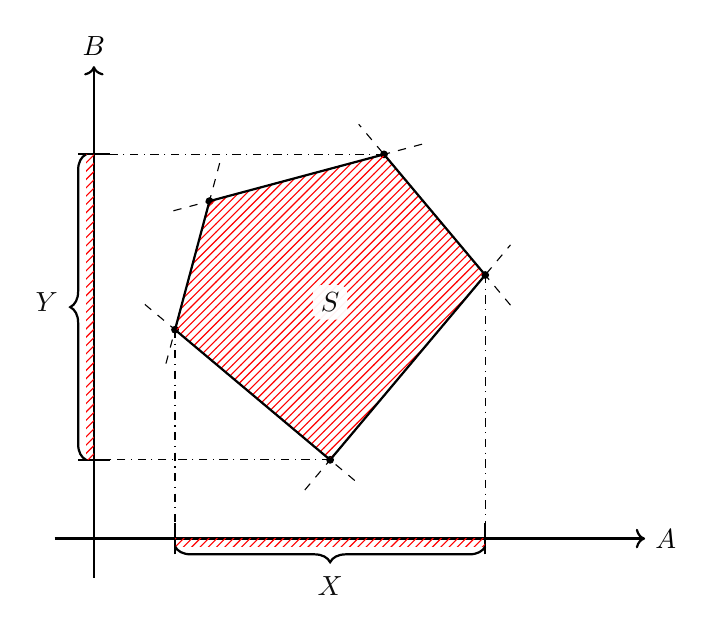
\begin{tikzpicture}[
        extend line/.style={dashed, shorten >= -0.5cm,shorten <= -0.5cm},
        set region/.style={pattern=north east lines, pattern color=red},
        set label/.style={rounded corners=1mm, inner sep=1mm, fill=white, fill opacity=0.95}
    ]
    \coordinate (ori) at (-3,-3);
    \coordinate (A) at ($(ori)+(+7,0)$);
    \coordinate (B) at ($(ori)+(0,+6)$);
    \draw[thick, ->, shorten <= -0.5cm] (ori) -- (A) node[right]{$A$};
    \draw[thick, ->, shorten <= -0.5cm] (ori) -- (B) node[above]{$B$};

    \coordinate (x1) at ( -90:2);
    \coordinate (x2) at ( +10:2);
    \coordinate (x3) at ( +70:2);
    \coordinate (x4) at (+140:2);
    \coordinate (x5) at (+190:2);
    \foreach \p in {x1,x2,x3,x4,x5} {
        \node at (\p)[circle,fill,inner sep=1pt]{};
        \coordinate (\p A) at ($(ori)!(\p)!(A)$);
        \coordinate (\p B) at ($(ori)!(\p)!(B)$);
    }
    \draw [thick, set region] (x1) -- (x2) -- (x3) -- (x4) -- (x5) -- cycle;
    \foreach \p/\q in {x1/x2,x2/x3,x3/x4,x4/x5,x5/x1} {
        \draw [extend line] (\p) -- (\q);
    }

    \foreach \p in {x2,x5} {
        \draw [dash dot] (\p) -- (\p A);
        \draw [thick] ([yshift=-2mm]\p A) -- ([yshift=+2mm]\p A);
    }
    \path[set region] (x5A) rectangle ([yshift=-1mm]x2A);

    \foreach \p in {x1,x3} {
        \draw [dash dot] (\p) -- (\p B);
        \draw [thick] ([xshift=-2mm]\p B) -- ([xshift=+2mm]\p B);
    }
    \path[set region] (x3B) rectangle ([xshift=-1mm]x1B);
    \node[set label] at (0,0) {$S$};
    \node[set label] at ([yshift=-6mm]$(ori)!(0,0)!(A)$) {$X$};
    \node[set label] at ([xshift=-6mm]$(ori)!(0,0)!(B)$) {$Y$};

    \draw[thick,decorate,decoration={brace,amplitude=2mm}] ([yshift=-1mm]x2A) -- ([yshift=-1mm]x5A);
    \draw[thick,decorate,decoration={brace,amplitude=2mm}] ([xshift=-1mm]x1B) -- ([xshift=-1mm]x3B);
\end{tikzpicture}
\end{center}

\subsection{The Codomain Fibration}

\begin{defn}
    \label{def:arrow_category}
    For any category $\catC$, its \textbf{arrow category} $\arr(\catC)$ has as objects the morphisms $f : f_0 \to f_1$ of $\catC$ and has as morphisms $\alpha : f \to g$ the commuting squares of $\catC$, i.e.
    \begin{equation}
        \begin{tikzcd}[row sep=small, column sep=small]
            f_0 \ar[r, "f"] \ar[d, "\alpha_0"'] & f_1 \ar[d, "\alpha_1"] \\
            g_0 \ar[r, "g"'] & g_1
        \end{tikzcd}
    \end{equation}
\end{defn}
The arrow category can be equivalently defined as a functor category $[\mathsf{I}, \catC] \simeq \arr(\catC) = \catC^{\mathsf{I}}$ where $\mathsf{I}$ is the \textit{interval category}
\begin{equation}
    \begin{tikzcd}
        0 \ar[loop left, "\id_{0}"] \ar[r, "i"] & 1 \ar[loop right, "\id_{1}"]
    \end{tikzcd}
\end{equation}
consisting of two objects and a non-identity morphism $i : 0 \to 1$ between them.

\begin{defn}
    The \textbf{codomain functor} $\cod : \arr(\catC) \to \catC$ takes a morphism of $\arr(\catC)$ (commuting square of $\catC$) $\alpha : f \to g$ to its codomain $\cod (\alpha) = g$,
    \begin{equation}
        \cod \left(
            \begin{tikzcd}[row sep=small, column sep=small]
                f_0 \ar[r, "f"] \ar[d, "\alpha_0"'] & f_1 \ar[d, "\alpha_1"] \\
                g_0 \ar[r, "g"'] & g_1
            \end{tikzcd}
        \right)
        =
        \begin{tikzcd}[column sep=small]
            g_0 \ar[r, "g"'] & g_1
        \end{tikzcd}
    \end{equation}
\end{defn}

The fibers of the codomain functor $\cod : \arr(\catC) \to \catC$ are therefore isomorphism to the slice categories; given an object $a$ in $\catC$, the fiber over $a$ is the slice category $\arr_{a}(\catC) \simeq \catC / a$ whose morphisms are commuting triangles over $a$ in $\catC$, i.e.
\begin{equation}
    \begin{tikzcd}[column sep=small]
        c \ar[dr, "g"'] \ar[rr, "t"] & & d \ar[dl, "h"] \\
        & a &
    \end{tikzcd}.
\end{equation}

Automatically, observe that the codomain functor $\cod : \arr(\catC) \to \catC$ constitutes an opfibration; for each morphism $f : a \to b$, the associated fiber-convariant functor $f_{!} : \catC / a \simeq \arr_{a}(\catC) \to \arr_{b}(\catC) \simeq \catC / b$ is specified by post-composition with $f$:
\begin{equation}
    f_! \left(
        \begin{tikzcd}[column sep=small]
            c \ar[dr, "g"'] \ar[rr, "t"] & & d \ar[dl, "h"] \\
            & a &
        \end{tikzcd}
    \right)
    =
    \begin{tikzcd}[column sep=small]
    c \ar[dr, "f g"'] \ar[rr, "t"] & & d \ar[dl, "f h"] \\
    & b &
    \end{tikzcd}
\end{equation}
\begin{equation}
    \begin{tikzcd}[sep=large]
        c \ar[d, "g"'] \ar[r, "t"] & d \ar[dl, "h", near end] \ar[d, "f h"] \\
        a \ar[r, "f"'] & b \ar[from=ul, "f g", near start, crossing over]
    \end{tikzcd}.
\end{equation}

Under the right conditions, a codomain functor is also a \textit{fibration} and thus an \textit{bifibration}.

\begin{prop}
    If a category $\catB$ has pullbacks, the codomain functor $\cod : \arr(\catB) \to \catB$ is a fibration called the \textbf{codomain fibration}.
\end{prop}
For each morphism $f : a \to b$ in the base $\catB$, the associated fiber-contravariant functor $f^{\ast} : \catB / a \to \catB / b$ is specified by pullback along $f$:
\begin{equation}
    f^\ast \left(
        \begin{tikzcd}[column sep=small]
            c \ar[dr, "g"'] \ar[rr, "t"] & & d \ar[dl, "h"] \\
            & b &
        \end{tikzcd}
    \right)
    =
    \begin{tikzcd}[column sep=small]
        c' \ar[dr, "f^\ast g"'] \ar[rr, "t'"] & & d' \ar[dl, "f^\ast h"] \\
        & b &
    \end{tikzcd}
\end{equation}
\begin{equation}
    \begin{tikzcd}[
            execute at end picture={
                \pullback{m-2-2}{m-2-4}{m-3-1};
                \pullback[line width=2mm, white]{m-1-1}{m-3-1}{m-1-3}; % options here allow for a "crossing under" effect
                \pullback{m-1-1}{m-3-1}{m-1-3};
            }
        ]
        c' \ar[dd, "f^\ast g"'] \ar[dr, dashed, "t'"] \ar[rr, "g^\ast f"] & & c \ar[dr, "t"] & \\
        & d' \ar[dl, "f^\ast h"] \ar[rr, "h^\ast f", near start] & & d \ar[dl, "h"] \\
        a \ar[rr, "f"'] & & b \ar[from=uu, "g"', crossing over, near end] &
    \end{tikzcd}.
\end{equation}
Note that the morphism $t' : c' \to d'$ completing the resulting commuting triangle is unique by the universality of $d'$ as the pullback of \begin{tikzcd}[cramped] a \ar[r, "f"] & b & d \ar[l, "h"'] \end{tikzcd}.

Given a category $\catB$ with pullbacks, and a morphism $f : a \to b$ of $\catB$, the codomain bifibration $\cod : \arr(\catB) \to \catB$ induces a adjoint pair of functors between the fibers
\begin{equation}
    \begin{tikzcd}
        \catB / a
        \arrow[r, bend left, "f_!", ""{name=L,inner sep=1pt,below}]
        \arrow[from=r, bend left, "f^\ast", ""{name=R,inner sep=1pt}]
        &
        \catB / b 
        \arrow[from=L, to=R, symbol=\dashv]
    \end{tikzcd}
\end{equation}
such that $f_! : \catB / a \to \catB / b$ is given by post-composition and $f^\ast: \catB / b \to \catB / a$ is given by pullback.

\begin{lem}
    Given a category $\catB$ with all pullbacks, the codomain bifibration $\cod : \arr(\catB) \to \catB$ satisfies the Beck-Chevalley condition at all pullback squares in $\catB$.
\end{lem}

\begin{proof}
    Consider an arbitrary pullback square in base category $\catB$,
    \begin{equation}
        \label{eq:generic_pullback}
        \begin{tikzcd}[execute at end picture={\pullback{m-1-1}{m-1-2}{m-2-1}}]
            a \ar[r, "f"] \ar[d, "h"'] & b \ar[d, "g"] \\
            c \ar[r, "k"'] & d
        \end{tikzcd}.
    \end{equation}
    Automatically, there exists a natural isomorphism $\alpha : f^\ast g^\ast \to h^\ast k^\ast$:
    \begin{equation}
        \label{eq:right_adjoint_square}
        \begin{tikzcd}
            \catB / a \ar[from=r, "f^\ast"'] \ar[from=d, "h^\ast"] & \catB / b \ar[from=d, "g^\ast"'] \ar[dl, Rightarrow, "\alpha"', "\simeq", sloped] \\
            \catB / c \ar[from=r, "k^\ast"] & \catB / d 
        \end{tikzcd}
    \end{equation}
    The individual components $\alpha_{\psi}$ for each object $\psi : p \to d$ of $\catB / d$ is specified by the following diagram:
    \begin{equation}
        \begin{tikzcd}[
                execute at end picture={
                    \pullback{m-1-3}{m-2-2}{m-2-4};
                    \pullback{m-1-1}{m-2-1}{m-1-3};
                    \pullback{m-1-5}{m-2-5}{m-1-3};
                    \pullback{m-2-1}{m-3-1}{m-2-2};
                    \pullback{m-2-5}{m-3-5}{m-2-4};
                }
            ]
            a' \ar[rr, "h^\ast k^\ast \psi"'] \ar[d] & & a \ar[dr, "f"'] \ar[dl, "h"] & & a'' \ar[ll, "f^\ast g^\ast \psi"] \ar[d]
            \ar[llll, bend right=25, dashed, "\alpha_{\psi}", "\simeq"'] \\ 
            c' \ar[r, "k^\ast \psi"] \ar[d] & c \ar[dr, "k"] & & b \ar[dl, "g"'] & b' \ar[l, "g^\ast \psi"'] \ar[d] \\ 
            p \ar[rr, "\psi"] \ar[rrrr, bend right=20, equals] & & d & & p \ar[ll, "\psi"'] \\
        \end{tikzcd}
    \end{equation}
    Using the composition of pullback squares, it is clear that \textit{both} $h^\ast k^\ast \psi$ and $f^\ast g^\ast \psi$ are projection morphisms (onto $a$) in the pullback square of \begin{tikzcd}[cramped] a \ar[r, "gf = kh"] & d & p \ar[l, "\psi"'] \end{tikzcd} and therefore, they are unique up to a unique isomorphism; the component $\alpha_{\psi}$ is precisely that isomorphism. Notice that this argument \textit{does not} make use of the fact that the original commuting square in Equation~\ref{eq:generic_pullback} was a pullback square.

    To prove the Beck-Chevalley condition, one must demonstrate that the natural transformation $\beta = \varepsilon_{h} \alpha \eta_{g} : h_! f^\ast \to k^\ast g_!$ is also a \textit{natural isomorphism}. Remembering that the left adjoints can be computed by post-composition, the component of $\beta$ for an object $\psi : p \to b$ of $\catB / b$, denoted $\beta_{\psi}$, and its inverse can be determined by the following diagram:
    \begin{equation}
        \begin{tikzcd}[
                execute at end picture={
                    \pullback{m-1-1}{m-2-1}{m-1-2};
                    \pullback{m-1-4}{m-1-3}{m-2-4};
                    \pullback{m-1-3}{m-1-2}{m-2-3};
                }
            ]
            c' \ar[r, "k^\ast g_! \psi"] \ar[d]\ar[from=rrr, bend right=50, dashed, "\beta_{\psi}", "\simeq"'] & c \ar[d, "k"] & a \ar[l, "h"'] \ar[d, "f"]  & a' \ar[l, "f^\ast \psi"'] \ar[ll, bend right, "h_! f^\ast \psi"'] \ar[d] \\
            p \ar[r, "g_! \psi"] \ar[rrr, bend right=15, equals] & d & b \ar[l, "g"'] & p \ar[l, "\psi"']
        \end{tikzcd}
    \end{equation}
    Similarly, $k^\ast g_! \psi$ and $h_! f^\ast \psi$ are \textit{both} projection morphisms (onto $c$) in the pullback square of \begin{tikzcd}[cramped] p \ar[r, "g\psi"] & d & c \ar[l, "k"'] \end{tikzcd} and therefore, they are unique up to a unique isomorphism $\beta_{\psi}$. The key difference in this case is that this argument \textit{does} rely on $a$ being the pullback object in the original pullback square in the base $\catB$ (Equation~\ref{eq:generic_pullback}).
\end{proof}

\subsection{The Subobject Fibration}

\subsubsection{Definitions}

Given any category $\catB$, and an object $X$ of $\catB$, a \textit{subobject} of $X$ is an isomorphism class of monomorphisms $f : Y \hookrightarrow X$; two monomorphisms $f : Y \hookrightarrow X, g : Z \hookrightarrow
X$ with shared codomain $X$ are isomorphic if there exists an isomorphism $h : Y \xrightarrow{\sim} Z$ such that $f = g \circ h$. The individual monomorphisms of a subobject class can be equipped with a preorder relation $( f : Y \hookrightarrow X ) \leq ( g : Z \hookrightarrow X )$ if there exists $k : Y \rightarrow Z$ such that $f = g \circ k$:
\begin{equation}
    \begin{tikzcd}[column sep=small]
        Y \ar[rd, hook, "f"'] \ar[rr, "k"] &   & Z \ar[ld, hook', "g"]\\
          & X &
    \end{tikzcd}
\end{equation}
Note that if such a $k : Y \to Z$ exists, then it is unique because it $g$ is a monomorpism; if $k' : Y \rightarrow Z$ satisfied $f = g \circ k'$ as well, then $g \circ k = g \circ k'$ which implies $k = k'$. Moreover, this preorder relation on the individual monomorphisms extends to a poset $\sub_{\catB}(X)$ between the subobjects. For example, if $\catB$ is the category $\set$, the subobjects of $X$ are subsets of $X$ and thus $\sub_{\set}(X) \cong \pow(X)$. Even more concretely, if $X$ is the set $\mathbb{R}^2$, an exemplary diagram of $\sub_{\set}(\mathbb{R}^2)$ is
\begin{center}
    \begin{tikzcd}[column sep=small]
        & A & \\
        B \ar[ur, hook', "\subseteq"] & & C \ar[ul, hook, "\subseteq"'] \\
        & D \ar[ul, hook', "\subseteq"] \ar[ur, hook, "\subseteq"'] \ar[uu, hook, "\subseteq"] & \\
    \end{tikzcd}
    \hspace{3em}
    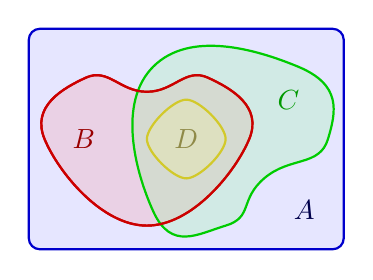
\begin{tikzpicture}[
            set border/.style={draw=#1!80!black},
            set region/.style={set border=#1, fill=#1!50!white, fill opacity=0.2},
            set label/.style={draw=#1!80!black}
        ]
        \draw[thick, set region=blue, rounded corners] (-2,-1.4) rectangle (+2, +1.4) {};

        \begin{scope}[shift={(-0.5,0)}]
            \coordinate (y1) at (  +0:1.3);
            \coordinate (y2) at ( +45:1.1);
            \coordinate (y3) at ( +90:0.6);
            \coordinate (y4) at (+135:1.1);
            \coordinate (y5) at (+180:1.3);
            \coordinate (y6) at (+270:1.1);
            \draw [thick, set region=red] plot [smooth cycle, tension=0.8] coordinates {(y1) (y2) (y3) (y4) (y5) (y6)};
        \end{scope}
        \begin{scope}[shift={(+0.5,0)}]
            \coordinate (z1) at ( +45:1.3);
            \coordinate (z2) at (+135:1.3);
            \coordinate (z3) at (+225:1.3);
            \coordinate (z4) at (+270:1.1);
            \coordinate (z5) at (+315:0.7);
            \coordinate (z6) at (+360:1.3);
            \draw [thick, set region=green] plot [smooth cycle, tension=0.9] coordinates {(z1) (z2) (z3) (z4) (z5) (z6)};
        \end{scope}
        \draw [thick, set border=red] plot [smooth cycle, tension=0.8] coordinates {(y1) (y2) (y3) (y4) (y5) (y6)};
        \coordinate (w1) at (  +0:0.5);
        \coordinate (w2) at ( +90:0.5);
        \coordinate (w3) at (+180:0.5);
        \coordinate (w4) at (+270:0.5);
        \draw [thick, set region=yellow] plot [smooth cycle, tension=0.6] coordinates {(w1) (w2) (w3) (w4)};

        \node at (+0,+0) {\color{yellow!50!black}$D$};
        \node at (+1.3,+0.5) {\color{green!60!black}$C$};
        \node at (-1.3,+0) {\color{red!60!black}$B$};
        \node at (+1.5,-0.9) {\color{blue!30!black}$A$};
    \end{tikzpicture}
\end{center}
If the category $\catB$ has pullbacks, the posetal categories $\sub_{\catB}(X)$ for varying objects $X$ of $\catB$ can be ``stitched together'' to form an enveloping category denoted $\sub(\catB)$. The objects of $\sub(\catB)$ are the objects of $\sub_{\catB}(X)$ for various $X$. The morphisms of $\sub(\catB)$ are defined using the morphisms of $\catB$. Given a equivalence class of monomorphisms $B = \{b_i : Z_i \hookrightarrow X \}_{i \in \mathcal I} \in \sub_{\catB}(X)$ with with shared codomain $X$, and morphism $f : Y \to X$ (not necessarily a monomorphism) with codmain $X$, the pullbacks $f^\ast b_i$ of $b_i$ along $f$ for each $i \in \mathcal I$ constitute an equivalence class of monomorphisms $f^{\ast}B \coloneqq \{f^{\ast} b_i : Y \times_{X} Z_i \hookrightarrow Y \}_{i \in \mathcal I} \in \sub_{\catB}(Y)$:\footnote{Evidently, this relies on the fact that pullbacks perserve monomorphisms; i.e. $b : Z \hookrightarrow X$ is a monomorphism, then the pullback $f^\ast b : Y \times_{X} Z \hookrightarrow Y$ is also.}\footnote{The isomoprhisms connecting the monomorphisms of $f^\ast B$ are also given by pullback of the isomorphisms connecting the monomorphisms of $B$.}
\begin{equation}
    \begin{tikzcd}
        Y \times_{X} Z_i \drpb{xshift=-2mm} \ar[r, "b_i^\ast f"] \ar[d, hook, "f^\ast b_i"'] & Z_i \ar[d, hook, "b_i"] \\
        Y \ar[r, "f"] & X
    \end{tikzcd}
\end{equation}
To every morphism $f : Y \to X$ of $\catB$, and object $B \in \sub_{\catB}(X)$, denote $\kappa_{f}(B) : f^\ast B \to B$ where $f^\ast B \in \sub_{\catB}(Y)$. Finally, a morphism of $\sub(\catB)$ between $A \in \sub_\catB(Y)$ and $B \in \sub_\catB(X)$ is the formal sequence \begin{tikzcd}[cramped] A \ar[r, "\leq"] &  f^{\ast}(B) \ar[r, "\kappa_f(B)"] & B \end{tikzcd}. The projection functor $P_{\catB} : \sub(\catB) \to \catB$ defines the \textit{subobject fibration}\footnote{Note that while the fibres $\sub_{\catB}(X)$ are thin, the total category $\sub(\catB)$ is not necessarily thin.}.

\ctodo{figure out the relationship between a subobject fibration and the codomain fibration via the notion of \href{https://math.stackexchange.com/questions/2171645/how-can-the-subobject-fibration-be-obtained-from-the-codomain-fibration/2173108}{subterminal objects}.}

\subsubsection{The Beck-Chevalley Condition}

Given any category $\catB$ with all pullbacks, the functor $P_{\catB} : \sub_{\catB} \to \catB$ which sends subobjects $[\psi]$ to their shared codomains, constitutes a bifibration. In particular, given a morphism $f : a \to b$ of $\catB$, there is an induced adjoint pair of functors between the subobject fibers:
\begin{equation}
    \begin{tikzcd}
        \sub_{\catB}(a)
        \arrow[r, bend left, "f_!", ""{name=L,inner sep=1pt,below}]
        \arrow[from=r, bend left, "f^\ast", ""{name=R,inner sep=1pt}]
        &
        \sub_{\catB}(b)
        \arrow[from=L, to=R, symbol=\dashv]
    \end{tikzcd}
\end{equation}
Specfically, left adjoint functor $f_{!}$ acting on a subobject $[\psi] : \sub_{\catB}(a)$ (where $[\psi]$ is the equivalence class of monomorphisms into $a$ containing $\psi : a' \hookrightarrow a$) is given by post-composition $f_{!} ( [\psi] ) = [ f \psi ] \in \sub_{\catB}(b)$ in $\catB$.
\tob{That works for the codomain fibration, but not here, because $f \psi$ is generally not a subobject. Rather, $f_! ( [\psi] )$ should be the \emph{image} of the morphism $f \psi$, in the sense of \href{https://ncatlab.org/nlab/show/image}{image factorization} (please check whether this works). Thus one needs to assume that image factorizations exist}
The right adjoint functor $f^\ast$ acting on a subobject $[\phi] \in \sub_{\catB}(b)$ is given by pullback of \begin{tikzcd}[cramped]a \ar[r, "f"]  & b & b' \ar[l, hook', "\phi"'] \end{tikzcd} in $\catB$:
\begin{equation}
    \begin{tikzcd}
        f^{*}b' \drpb{} \ar[r] \ar[d, hook, "f^\ast \phi"'] & b' \ar[d, hook, "\phi"] \\
        a \ar[r, "f"'] & b
    \end{tikzcd}
\end{equation}

Generally speaking, it is important to determine how diagrams in the base category $\catB$ behave when lifted to the total category $\sub_{\catB}$ under the associated pseudo-functors. For example, given a pullback square in base category $\catB$,
\begin{equation}
    \begin{tikzcd}
        a \drpb{} \ar[r, "f"] \ar[d, "h"'] & b \ar[d, "g"] \\
        c \ar[r, "k"'] & d
    \end{tikzcd}
\end{equation}
There exists a natural isomorphism $\alpha$ between the functors $f^\ast g^\ast$ and $h^\ast k^\ast$:
\begin{equation}
    \begin{tikzcd}
        \sub_{\catB}(a) \ar[from=r, "f"'] \ar[from=d, "h"] & \sub_{\catB}(b) \ar[from=d, "g"'] \ar[dl, Rightarrow, "\alpha", "\sim"'] \\
        \sub_{\catB}(c) \ar[from=r, "k"] & \sub_{\catB}(d)
    \end{tikzcd}
\end{equation}
The existence of components $\alpha_{[\psi]}$ for the subobject class containing the monomorphism $\psi : p \hookrightarrow d$ can be determined by examining the following diagram:
\begin{equation}
    \begin{tikzcd}
        & & & f^\ast g^\ast p \ar[d] \ar[lld, hook, out=180, in=90, "f^\ast g^\ast \psi"', near start] \dlpb{} \\
        & a \ar[r, "f"] \ar[d, "h"'] \drpb{} & b \ar[d, "g"] & g^\ast p \ar[l, "g^\ast \psi"', hook] \ar[dd] \dlpb{} \\
        & c \ar[r, "k"'] & d & \\
        h^\ast k^\ast p \ar[r] \ar[uur, hook, out=90, in=180, "h^\ast k^\ast \psi", near start] \urpb{} & k^\ast p \ar[u, hook, "k^\ast \psi"] \ar[rr] \urpb{} & & p \ar[ul, hook, "\psi"']
    \end{tikzcd}
\end{equation}
Using the composition of pullback squares, it is clear that \textit{both} $f^\ast g^\ast p$ and $h^\ast k^\ast p$ are pullbacks of \begin{tikzcd}[cramped] a \ar[r, "gf = kh"] & d & p \ar[l, hook', "\psi"'] \end{tikzcd} and therefore, they are unique up to a unique isomorphism which will be denoted $\beta$. It is important to notice that this does not depend on $a$ being a pullback itself.
\begin{equation}
    \begin{tikzcd}[row sep=large]
        h^\ast k^\ast p
        \ar[d, hook', "h^\ast k^\ast \psi"']
        \ar[rrd, bend left]
        \ar[rr, bend left, dashed, "\beta^{-1}"']
        \drpb{}
        &
        &
        f^\ast g^\ast p
        \ar[d]
        \ar[lld, bend right, hook', "f^\ast g^\ast \psi", near end]
        \ar[ll, bend right=40, dashed, "\beta"']
        \dlpb{}
        \\
        a
        \ar[r, "gf=kh"']
        &
        d
        &
        p
        \ar[l, hook', "\psi"]
    \end{tikzcd}
\end{equation}
These isomorphisms actually establish that $h^\ast k^\ast \psi \simeq f^\ast g^\ast \psi$ and therefore they belong to the same equivalence class $[h^\ast k^\ast \psi] = [ f^\ast g^\ast \psi ]$ for each $\psi$. Therefore, it becomes clear that the natural isomorphism is indeed the identity natural transformation $\id_{f^\ast g^\ast} = \id_{h^\ast k^\ast} = \alpha : f^\ast g^\ast \to h^\ast k^\ast$.\footnote{Ultimately, the reason for $\alpha = \id$ is due to considering $\sub_{\catB}(a)$, the \textit{poset} of subobjects of $a$, instead of $\mono_{\catB}(a)$ the \textit{preorder} of monomorphisms into $a$.}

Alternatively, one can consider whether or not there exists natural transformations (or natural isomorphisms) of the form $\alpha : h_! f^\ast \to k^\ast g_!$. Remembering that the left adjoints $f_{!}$ are specified by post-composition $f_{!} [\psi] \to [f \psi]$, this question can be answered by considering the following diagram:
\begin{equation}
    \begin{tikzcd}
        k^\ast g p \ar[r, "k^\ast g \psi"] \ar[d] \drpb{} & c \ar[d, "k"] & a \ar[l, "h"] \ar[d, "f"] \dlpb{} & f^\ast p \ar[l, "f^\ast \psi", hook'] \ar[ll, bend right, "h f^\ast \psi"'] \ar[d] \dlpb{} \\
        p \ar[r, "g\psi"] \ar[rrr, bend right=15, equals] & d & b \ar[l, "g"'] & p \ar[l, hook', "\psi"']
    \end{tikzcd}
\end{equation}
Similarly, $k^\ast g p$ and $f^\ast p$ are \textit{both} pullbacks of \begin{tikzcd}[cramped] p \ar[r, "g\psi"] & d & c \ar[l, hook', "k"'] \end{tikzcd} and therefore, we obtain an analogous statement: since $h f^\ast \psi \simeq k^\ast g \psi$, we have $[h f^\ast \psi] = [k^\ast g \psi]$ and therefore $h_! f^\ast = k^\ast g_!$.
\tob{Nice! Even though the pushforward functors are missing the image factorizations, I think that this is the correct argument in the case of the codomain fibration. For the subobject fibration, we might need some additional stability property, presumably the one stated in the alternative definition of \href{https://ncatlab.org/nlab/show/regular+category\#definition}{regular categories}}
The key difference in this case is that this argument \textit{does} rely on $a$ being the pullback of a pullback square.

In summary, the subobject fibration \textit{satisfies} the Beck-Chevalley condition. Moreover, since none of the above argument relies on the fact that the objects of total category are represented by \textit{monomorphisms} in the base, just that they correspond to \textit{morpisms} in the base, it is clear that any codomain bifibration also satisfies the Beck-Chevalley condition.

\subsection{The Category of Convex Cones and Linear Maps}

Given any $\mathbb{R}$-vector space $V$, a \textit{(closed) cone} $C \subseteq V$ is a subset of $V$ such that for any elements $c_1, c_2 \in C$ and for any positive coefficients $\gamma_1, \gamma_2 \geq 0$, $\gamma_1 c_1 + \gamma_2 c_2 \in C$. A polyhedral cone $C \subseteq V$ is one which admits a half-space representation in terms a finite number of linear constraints:
\begin{equation}
    C = \{ x \in V \mid \bigwedge_{i=1}^{K} (a_i \cdot x \geq 0) \}
\end{equation}
Alternatively, a $\cone$ can be expressed in terms of the pullback of the positive orthant
\begin{equation}
    \mathbb{R}_{+}^{n} \coloneqq \{v \in \mathbb{R}^n \mid \forall i \in [n]: v_i \geq 0 \}
\end{equation}
by a linear transformation $f : V \to \mathbb{R}^{n}$ into $\mathbb{R}^{n}$.
\begin{equation}
    \begin{tikzcd}
        f^{*}(\mathbb{R}^n_+) \drpb{xshift=-2mm} \ar[r] \ar[d, hook] &  \mathbb{R}^n_+ \ar[d, hook, "i_+"] \\
        V \ar[r, "f"] & \mathbb{R}^n
    \end{tikzcd}
\end{equation}
\begin{equation}
    f^{*}(\mathbb{R}^n_+) \cong \{ v \in V \mid f(v) \in \mathbb{R}^n_+ \}
\end{equation}
Given a cone $f^{*}(\mathbb{R}^n_+) \subseteq V$ associated with a finite set of $n$ linear expressions $f : V \to \mathbb{R}^n$, and a linear transformation $g : V \to W$,

\subsection{Subset Projection}
A prototypical example wherein an adjoint triple
\[ f_{!}, \exists_{f} \dashv f^{\ast}, f^{-1} \dashv f^{!}, \forall_{f} \]
arises is that of functions $f : X \to Y$ between sets $X$ and $Y$. The inverse image functor $f^{\ast} : \mathscr{P}Y \to \mathscr{P}X$ is defined on a subset $T \subseteq Y$
\[ f^{\ast} ( T ) = \{ x \in X : f(x) \in T \}, \]
and is functorial in the sense that if $T \subseteq T' \subseteq Y$ then $f^{\ast}(T) \subseteq f^{\ast}(T') \subseteq f^{\ast}(T)$. The adjoint functors $\exists_{f}, \forall_{f} : \mathscr{P}X \to \mathscr{P}Y$ are defined on $S \subseteq X$ as
\begin{align*}
    \exists_{f} (S) &= \{ y \in Y : \exists x \in f^{\ast}(y) : x \in S \} \\
    \forall_{f} (S) &= \{ y \in Y : \forall x \in f^{\ast}(y) : x \in S \}
\end{align*}
form an adjoint triple in the sense that $\exists_{f} \dashv f^{\ast} \dashv \forall_{f}$:
\begin{align*}
    \exists_{f} \dashv f^{\ast} : \quad \exists_{f} (S) \subseteq T &\iff S \subseteq f^{\ast}(T) \\
    f^{\ast} \dashv \forall_{f} : \quad f^{\ast}(T) \subseteq R &\iff T \subseteq \forall_{f}(R)
\end{align*}

\begin{center}
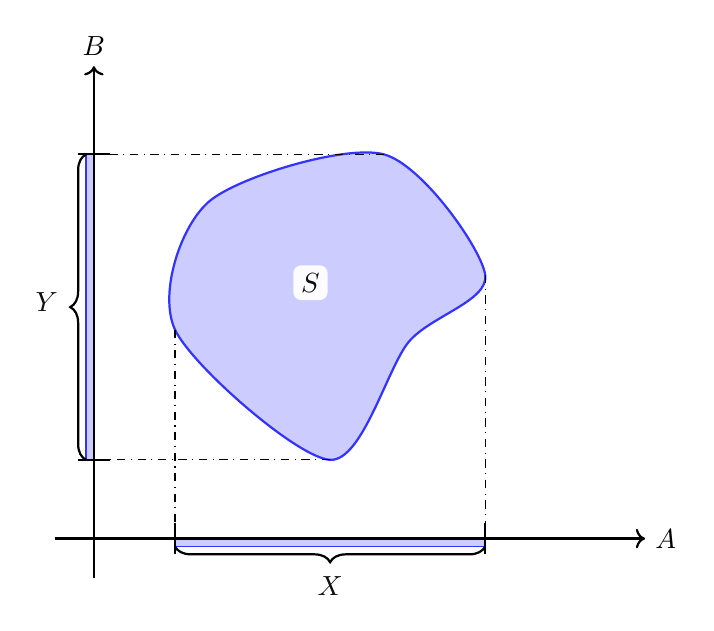
\begin{tikzpicture}[
        set region/.style={draw=blue!80, fill=blue!20},
        set label/.style={rounded corners=1mm, inner sep=1mm, fill=white, fill opacity=0.95}
    ]
    \coordinate (ori) at (-3,-3);
    \coordinate (A) at ($(ori)+(+7,0)$);
    \coordinate (B) at ($(ori)+(0,+6)$);

    \coordinate (x1) at ( -90:2);
    \coordinate (x2) at ( +10:2);
    \coordinate (x3) at ( +70:2);
    \coordinate (x4) at (+140:2);
    \coordinate (x5) at (+190:2);
    \foreach \p in {x1,x2,x3,x4,x5} {
        \coordinate (\p A) at ($(ori)!(\p)!(A)$);
        \coordinate (\p B) at ($(ori)!(\p)!(B)$);
    }
    \draw [thick, set region] plot [smooth cycle] coordinates {(x1) (+1,-0.5) (x2) (x3) (x4) (x5)};

    \path[set region] (x5A) rectangle ([yshift=-1mm]x2A);
    \path[set region] (x3B) rectangle ([xshift=-1mm]x1B);

    \foreach \p in {x2,x5} {
        \draw [dash dot] (\p) -- (\p A);
        \draw [thick] ([yshift=-2mm]\p A) -- ([yshift=+2mm]\p A);
    }

    \foreach \p in {x1,x3} {
        \draw [dash dot] (\p) -- (\p B);
        \draw [thick] ([xshift=-2mm]\p B) -- ([xshift=+2mm]\p B);
    }
    \node[set label] at (-0.25,+0.25) {$S$};

    \node[set label] at ([yshift=-6mm]$(ori)!(0,0)!(A)$) {$X$};
    \node[set label] at ([xshift=-6mm]$(ori)!(0,0)!(B)$) {$Y$};

    \draw[thick,decorate,decoration={brace,amplitude=2mm}] ([yshift=-1mm]x2A) -- ([yshift=-1mm]x5A);
    \draw[thick,decorate,decoration={brace,amplitude=2mm}] ([xshift=-1mm]x1B) -- ([xshift=-1mm]x3B);

    \draw[thick, ->, shorten <= -0.5cm] (ori) -- (A) node[right]{$A$};
    \draw[thick, ->, shorten <= -0.5cm] (ori) -- (B) node[above]{$B$};
\end{tikzpicture}
\end{center}

Consider a pair of sets $A$ and $B$ and a subset $S \subseteq A \times B$ of their cartesian product.  The projection morphisms associated with $A \times B$ are $p : A\times B \to A$ and $q : A \times B \to B$. The projection of the subset $S$ onto $A$ is then the subset $X \subseteq A$ defined by:
\[ X = \{ a \in A \mid \exists s \in S, p (s) = a \} \]

\begin{equation}
    S \subseteq p^{\ast} ( X ) \Longleftrightarrow \exists_p ( S ) \subseteq X
\end{equation}

\subsection{Optimization of real-valued functions}
\begin{center}
    \includegraphics[]{figures/min_max_multivariate_function/figure.pdf}
\end{center}

\section*{Potentially Annotated Bibliography}
This section is temporary and reserved for recording comments toward various references.
\begin{itemize}
    \item \citeauthor{vistoli2004notes}~\cite{vistoli2004notes}
    \item \citeauthor{street1974fibrations}~\cite{street1974fibrations}
    \item \citeauthor{koudenburg2018categorical}~\cite{koudenburg2018categorical}
    \item \citeauthor{brown2009algebraic}~\cite{brown2009algebraic}
    \item \citeauthor{lurie2009higher}~\cite{lurie2009higher}
    \item \citeauthor{shulman2008framed}~\cite{shulman2008framed}
    \item \citeauthor{boyd2004convex}~\cite{boyd2004convex}
    \item \citeauthor{bogart2013hom}~\cite{bogart2013hom}
    \item \citeauthor{gubeladze2016affine}~\cite{gubeladze2016affine}
    \item \citeauthor{fausk2003isomorphisms}~\cite{fausk2003isomorphisms}
    \item \citeauthor{hofstra2011dialectica}~\cite{hofstra2011dialectica}
    \item \citeauthor{ponto2012duality}~\cite{ponto2012duality}
    \item \citeauthor{mac2013categories}~\cite{mac2013categories}
    \item \citeauthor{ziegler2012lectures}~\cite{ziegler2012lectures}
    \item \href{https://en.wikipedia.org/wiki/Spectrahedron}{Spectrahedron} are interesting semi-algebaric sets. (\url{https://www.youtube.com/watch?v=AevFRN5sxOU}).
\end{itemize}

% === [Bibliography] ===
\printbibliography

\end{document}
